%\documentclass[draftclsnofoot,onecolumn]{IEEEtran}
\documentclass[3p]{elsarticle}
\usepackage{tipa}
\usepackage{amsmath}%math
\usepackage{amsthm}%proof
\usepackage{xcolor}%color
\usepackage{bm}
\usepackage{graphicx}
\usepackage{booktabs}
\usepackage{textcomp}
\usepackage[colorlinks,linkcolor=black,anchorcolor=black,citecolor=black]{hyperref}
\usepackage{amsfonts,amssymb}
\usepackage{color,soul}
\theoremstyle{plain}
\newtheorem{myas}{Assumption}
\newtheorem{mydef}{Definition}
\newtheorem{mylem}{Lemma}
\newtheorem{mythm}{Theorem}

%\theoremstyle{remark}
\theoremstyle{remark}
\newtheorem{myrem}{Remark}

\begin{document}
\begin{frontmatter}
\title{A New Dual Terminal Sliding Mode Control Design For Rigid Robotic Manipulator}
\author{Zhiqiang Ma}
\author{Guanghui Sun\corref{cor1}}
\ead{guanghuisun@hit.edu.cn}
\cortext[cor1]{Corresponding author}
\address{Research Institute of Intelligent Control and Systems, Harbin Institute of Technology, Harbin 150001, China}

\begin{abstract}
This paper proposes a novel dual terminal sliding mode control for rigid robotic manipulator. A new terminal sliding mode manifold design technique is addressed to achieve finite time convergence of the sliding phase, and furthermore utilizing the involved dual variables combines the individual sliding mode surfaces to obtain an integral sliding mode dynamics, the convergence time of which is also integral for the entire system. The underactuated issue is coped with by introducing the hierarchical sliding mode methodology into the basic dual sliding mode design. These newly proposed methods also have the characteristics of nonsingularity and chattering suppression, and the effectiveness and high efficiency are verified by stabilizing the motions of the overhead crane and the rigid robotic manipulator. Simulation results validate the theoretical analysis about the proposed method.
\end{abstract}
\begin{keyword}
Finite time control; Robotic manipulator control; Terminal sliding mode; Sliding mode manifold design; Stability analysis
\end{keyword}
\end{frontmatter}
\section{Introduction}
Variable structure systems (VSS) are best known due to their insensitivity to parameter variations and uncertainties~\cite{slotine1991applied}. Its widely utilization in reality, such as DC and AC motors, process control, aircrafts, satellites, robots and so on, has validated robustness of VSS. As one of the most important branch of the VSS, the sliding mode control (SMC) has become a popular solution to the issue about various control and signal process missions in recent years~\cite{zhao2015nonlinear,zhang2015attitude}. Meza-S{\'a}nchez et al. applied the second-order sliding mode controller to a 3-DOF helicopter prototype, and verified the effectiveness via the experimental test bed~\cite{meza2015output}. Zheng et al. implemented the SMC to eliminate the effect of the input quantization generated between the coder and the decoder~\cite{zheng2016sliding}. Guzman et al. investigated the application of a SMC in a power factor rectifier with constant switching frequency~\cite{guzman2016sliding}. Said et al. designed a robust adaptive sliding mode method to guarantee the asymptotically stability of a boost converter~\cite{oucheriah2013pwm}. Roughly speaking, the SMC scheme is competent for normal scientific mission, due to its insensitivity of parameters and uncertainties in system, however, there still exist some obstacles, such as noncontinuous switching input in high frequency and convergence speed design~\cite{boiko2013chattering,lee2009chattering}, preventing it from being utilized in some practical engineering cases~\cite{fridman2011sliding}. \par
For alleviating the side effects, many researchers addressed remarkable approaches to improve the performance of the SMC scheme in last decade~\cite{zong2013quasi,santiesteban2013time,mu2015continuous,evangelista2013lyapunov,gonzalez2014chattering,dadras2012fractional,zhao2013output}. Among these methods, the high-order sliding mode control and super-twisting sliding mode control effort to generate the continuous inputs~\cite{castillo2015higher,palosz2015laser,edwards2016adaptive,zhao2015finite,liu2015second}, which eliminate the chattering by hiding the switching in high-order terms or absorbing the switching via some techniques. \par
Besides the issue on repressing the chattering, the fast convergence of the SMC scheme is also a hot subject. Normal linear sliding mode control takes two steps to solve a problem about the stability, namely, conducting the system states onto the prescript sliding manifold and driving these states to the origin along the manifold, and some accelerating operations usually occur in this two phases. The first step is said to be the approaching phase which usually requires the states converge to the desired manifold in finite time, and selecting suitable Lyapunov function and control parameters may accelerate this process; the second step is the sliding phase which is related to the designed manifold closely, and trivial manifold design techniques are able to guarantee the asymptotically convergence. For achieving a fast convergence in the sliding phase, the terminal sliding mode (TSM) control is developed based on the finite time control theory~\cite{haimo1986finite,bhat1997finite}, and comparing with the sliding mode control design mentioned above, the most significant contributions of the terminal sliding mode is introducing the finite time convergence to the sliding phase to complete the global finite time convergence. Owing to the global finite time convergence, the terminal sliding mode control has been utilized to achieve the high precise control, i.e., in~\cite{li2015robust}, an adaptive TSM scheme controlled a $2$-link robotic manipulator to track the variable signal. Feng et al. presented a global terminal sliding mode algorithm for manipulating the rigid robot, and produced the control design by using Lagrangian dynamic expression~\cite{feng2002non}. In~\cite{kamal2016continuous}, Kamal addressed a continuous homogeneous sliding mode algorithm for a perturbed second-order plant, and the algorithm could be regarded as a combination of terminal and super-twisting sliding-mode, providing a convergence control in finite time. \par
According to the achievements mentioned above, one can find that the conventional terminal sliding mode manifold design techniques are similar, since they are all based on the single variable finite time control, in another words, the sliding mode dynamics only involves the individual variable and its derivative essentially~\cite{mu2016switching}. This nature makes the TSM scheme become an individual control subsystem, which leads to the complicity of global convergence time in some extent. In this paper, an integral sliding mode manifold technique is proposed for finite time stability of the second-order system, and the novel manifold involves two variables to guarantee the integral finite time convergence, and the convergence time is obtained easily. Also, the nonsingularity and chattering suppression are available in the scheme. \par
In this paper, a dual terminal sliding mode (DTSM) controller is proposed for a class of second-order nonlinear systems with disturbances and uncertainties. A novel DTSM manifold is exploited to fulfill the finite time convergence, and the approaching and sliding time are both able to be calculated directly. For coping with the underacutated issue, cooperating with the hierarchical sliding surface design methodology, we develop a hierarchical dual terminal sliding mode (HDTSM) control. A modified DTSM (MDTSM) control scheme is presented to stabilize the motion of the $n$-link robotic manipulators. The remained paper is organized as follows: Section~\ref{sec:2} introduces a DTSM scheme for a class of second-order system, and the finite time convergence of the approaching and sliding phase is verified. In addition, we add performance parameters for improving the DTSM scheme to obtain the MDTSM scheme, and the newly presented method has a better performance in theoretical analysis; for stabilizing the underactuated system, the HDTSM design is developed as well in this section. In Section~\ref{sec:3}, the MDTSM is applied to the motion regulation of the $n$-link robotic  manipulator, and the stability analysis is also carried out. Section~\ref{sec:4} exhibits the simulation results, and finally the conclusion is assigned in Section~\ref{sec:5}.
\section{Dual terminal sliding mode control}\label{sec:2}
Consider a second-order nominal nonlinear system:
\begin{align}
\begin{split}
\dot x_1(t) &= x_2(t)\\
\dot x_2(t) &= f_1(\bm x,t)+g_1(\bm x,t)+b_1(\bm x,t)u_1(t)\\
\dot x_3(t) &= x_4(t)\\
\dot x_4(t) &= f_2(\bm x,t)+g_2(\bm x,t)+b_2(\bm x,t)u_2(t),\label{eq:second-order system}
\end{split}
\end{align}
where $\bm x = [x_1,x_2,x_3,x_4]^T$ is the system vector state; $f(\bm x,t)$ and $b(\bm x,t)\neq 0$ are smooth nonlinear functions with respect to $\bm x$; $u_i(t)$, $i=1,2$ stands for the scalar input; $g_i(\bm x,t)$, $i=1,2$  is defined as a bounded nonlinear function which satisfies $\Vert g_i(\bm x,t)\Vert\le l_i$, $l_i>0, i=1,2$, meaning the uncertainty and disturbance of the system. For the system mentioned above, we can establish a desired dual terminal sliding manifold as:
\begin{align}
\bm s(t) = [s_1(t),s_2(t)]^T,
\end{align}
where
\begin{align}
\begin{split}
s_1(t) &= x_2(t)+\vert x_1(t)\vert^{\alpha} sgn(x_1(t))+x_1^3(t)-x_3(t)\\
s_2(t) &= x_4(t)+\vert x_3(t)\vert^{\alpha} sgn(x_3(t))+x_3^3(t)+x_1(t),\label{eq:dual sliding manifold}
\end{split}
\end{align}
where $sgn(x)$ is the sign function, and $0<\alpha<1$ is a positive constant. For the sake of simplicity, the symbol $t$ is usually omitted in this paper, which does not cause any confusion, and it will appear once the derivation concerns for the factor of the time strictly, i.e., the desired sliding manifold $\bm s(t)$ is often abbreviated to $\bm s$.\par
There exist two lemmas about the finite convergence theory, providing convergence forms which contribute to the verification of the finite time convergence about the DTSM control.
\begin{mylem}
As described in~\cite{moulay2006finite}, it's assumed that the continuous function $V(t)$ is positive-define, satisfying the following condition:
\begin{align}
\dot V(t)\le -dV^\beta(t)\quad\forall t\ge t_0, V(t_0)\ge 0,
\end{align}
where $d$ is a positive scalar, and $0<\beta<1$. Then the function $V(t)$ converges to the origin for any given $t_0$, and typically the finite convergence time $t_r$ can be given as follows:
\begin{align}
t_r \le t_0+\frac{V^{1-\beta}(t_0)}{d(1-\beta)}.
\end{align}\label{lemma:1}
\end{mylem}
\begin{mylem}
Consider a second-order system:
\begin{align}
\begin{split}
\dot x_1&=-\vert x_1\vert^\alpha sgn(x_1)-x_1^3+x_2\\
\dot x_2&=-\vert x_2\vert^\alpha sgn(x_3)-x_2^3-x_1,\label{eq:normal sliding manifold}
\end{split}
\end{align}
and selecting $V(t) = \frac{x_1^2+x_2^2}{2}$ obtains the finite convergence time as follows~\cite{moulay2006finite}:
%since $\vert x\vert-x^\alpha+\vert x\vert \ge 0,0<\alpha<1$
\begin{align}
%t_s\le t_0+\frac{2(x_1^2+x_2^2)^{1-\alpha}}{1-\alpha}
t_s\le t_0+\frac{(2V(t_0))^{\frac{1-\alpha}{2}}}{1-\alpha},
\end{align}
where the definitions of  $t_s$, $t_0$, $\alpha$ are similar to Lemma \ref{lemma:1}. Introducing the amplitude scalar $d$ into the Eqs.~(\ref{eq:normal sliding manifold}) obtains  more normal forms:
\begin{align}
\dot x_1&=-d(\vert x_1\vert^\alpha sgn(x_1)-x_1^3+x_2)\\
\dot x_2&=-d(\vert x_2\vert^\alpha sgn(x_2)-x_2^3-x_1),\label{eq:more normal sliding manifold}
\end{align}
the convergence time of which is
\begin{align}
t_s\le t_0+\frac{(2V(t_0))^{\frac{1-\alpha}{2}}}{d(1-\alpha)}.
\end{align}\label{lemma:2}
\end{mylem}
For stabilization of the second-order system shown as~Eq. (\ref{eq:second-order system}), DTSM control inputs are addressed according the following theorem.
\begin{mythm}\label{theorem:1}Dual Terminal Sliding Mode Control Design.
The second-order system (\ref{eq:second-order system}) will reach the desired manifold $\bm s = 0$ shown in~Eq. (\ref{eq:dual sliding manifold}) in finite time. The states of the system will converge to zero along the manifold $\bm s=0$ in finite time, if the inputs are designed as follows:
\begin{align}
\begin{split}
u_1 &= -b_1^{-1}(\bm x)(f_1(\bm x)+\alpha\vert x_1\vert^{\alpha-1}x_2+3x_1^2x_2-x_4+k_1sgn(s_1))\\
u_2 &= -b_2^{-1}(\bm x)(f_2(\bm x)+\alpha\vert x_3\vert^{\alpha-1}x_4+3x_3^2x_4+x_2+k_2sgn(s_2)),\label{eq:DSM input}
\end{split}
\end{align}
where $k_i = l_i+\eta_i$, $i=1,2$; $\eta_i>0$ is a positive scalar value.
\end{mythm}
\begin{proof}
According to the equivalent control technique and the sliding surface reaching condition~\cite{Arie1993sliding}, the inputs can be design as
\begin{align}\begin{split}
u_1 &= u_{eq1}+u_{sw1}\\
u_2 &= u_{eq2}+u_{sw2}\notag
\end{split}\end{align}
where
\begin{align}\begin{split}
u_{eq1} &= -b_1^{-1}(\bm x)(f_1(\bm x)+\alpha\vert x_1\vert^{\alpha-1}x_2+3x_1^2x_2-x_4)\\
u_{eq2} &= -b_2^{-1}(\bm x)(f_2(\bm x)+\alpha\vert x_3\vert^{\alpha-1}x_4+3x_3^2x_4+x_2)\notag
\end{split}\end{align}
are the eauivalent control inputs to ensure $\dot s_1 = 0$ and $\dot s_2=0$, respectively, with $u_i = u_{eqi}$, $i=1,2$. The switching inputs are designed as $u_{swi}=-b_i^{-1}k_isgn(s_i)$, $i=1,2$ to guarantee the finite time reaching conditions of the ideal sliding surface.

Consider the Lyapunov function $V=\frac{1}{2}{\bm s}^T\bm s$, the derivative of which with respect to time $\dot V = {\bm s}^T \bm {\dot s}$ follows
\begin{align}
\begin{split}
\dot V &= {\bm s}^T\dot{\bm  s}\\
&=s_1\dot s_1+s_2\dot s_2\\
&=s_1(f_1(\bm x)+g_1(\bm x)+b_1(\bm x)u_1+\alpha\vert x_1\vert^{\alpha-1}x_2+3x_1^2x_2-x_4)\\
&\quad +s_2(f_2(\bm x)+g_2(\bm x)+b_2(\bm x)u_2+\alpha\vert x_3\vert^{\alpha-1}x_4+3x_3^2x_4+x_2).\label{eq:V_1}
\end{split}
\end{align}
Substituting inputs (\ref{eq:DSM input}) in~Eq. (\ref{eq:V_1}) yields
\begin{align*}
\dot V &= s_1(-k_1sgn(s_1)+g_1(\bm x))+s_2(-k_2sgn(s_2)+g_2(\bm x))\\
&= -\eta_1s_1sgn(s_1)-\eta_2s_2sgn(s_2)+(g_1(\bm x)s_1 - l_1s_1sgn(s_1))+(g_2(\bm x)s_2 - l_2s_2sgn(s_2))\\
&= -\eta_1\vert s_1\vert-\eta_2\vert s_2\vert+(g_1(\bm x)s_1 - l_1\vert s_1\vert)+(g_2(\bm x)s_2 - l_2\vert s_2\vert)\\
&\le - \min(\eta_1,\eta_2)(\vert s_1\vert+\vert s_2\vert)\\
&\le -\min(\eta_1,\eta_2)({\bm s}^T\bm s)^\frac{1}{2}\\
&\le -\sqrt{2}\min(\eta_1,\eta_2)V^\frac{1}{2}\le 0.
\end{align*}
Hence, the system (\ref{eq:second-order system}) asymptotically converges to the desired manifold (\ref{eq:dual sliding manifold}), and incidentally the convergence time is calculated according to the finite time convergence theory.\par
Once the system (\ref{eq:second-order system}) reaches the desired manifold~(\ref{eq:dual sliding manifold}), the whole system is handled by the reduced system:
\begin{align*}
\dot x_1&=-\vert x_1\vert^\alpha sgn(x_1)-x_1^3+x_3\\
\dot x_3&=-\vert x_3\vert^\alpha sgn(x_3)-x_3^3-x_1.
\end{align*}\par
The total convergence time can be calculated by dividing the convergence into two phases with respect to the relation between the system and the manifold, namely, the approaching phase and the sliding phase, and specifically, according to Lemma \ref{lemma:2}, the total finite convergence time $t_f$ is calculated from:
\begin{align}
t_f = \underbrace{t_0+\frac{\sqrt{2}V^{\frac{1}{2}}(t_0)}{\min(\eta_1,\eta_2)}}_{t_r}+\underbrace{\frac{(2\hat V(t_r))^{\frac{1-\alpha}{2}}}{1-\alpha}}_{t_s}<\infty,
\end{align}
where $\hat V(t) = \frac{x_1^2+x_3^2}{2}$ is the Lyapunov function describing the convergence motion of the reduced system. The approaching and sliding time are defined as $t_r$ and $t_s$, respectively. This completes the proof.
\end{proof}
On the basis of Theorem \ref{theorem:1}, we proceed to develop the parameters in the manifold to improve the performance, which introduces a modified method for stabilizing the system~(\ref{eq:second-order system}), and furthermore this method makes the design of the manifold more flexible. Consider the system~(\ref{eq:second-order system}) with the manifold $\bm s = [s_1,s_2]^T$, the details of which are described by following expressions:
\begin{align}
\begin{split}
s_1(t) &= x_2(t)+\gamma(\vert x_1(t)\vert^{\alpha} sgn(x_1(t))+x_1^3(t))-\lambda x_3(t)\\
s_2(t) &= x_4(t)+\gamma(\vert x_3(t)\vert^{\alpha} sgn(x_3(t))+x_3^3(t))+\lambda x_1(t),\label{eq:modified dual sliding manifold}
\end{split}
\end{align}
where $\gamma$ is a positive constant and $\lambda\in R$ is a regulable parameter. Hence, the modified dual terminal sliding mode control inputs are formed in the following theorem.
\begin{mythm}\label{theorem:2}Modified Dual Terminal Sliding Mode Control Design.
The second-order system (\ref{eq:second-order system}) will reach the desired manifold $\bm s = 0$ shown in~Eq. (\ref{eq:modified dual sliding manifold}) in finite time. The states of the system will converge to zero along the manifold $\bm s=0$ in finite time, if the inputs are designed as follows:
\begin{align}
\begin{split}
u_1 &= -b_1^{-1}(\bm x)(f_1(\bm x)+\gamma\alpha\vert x_1\vert^{\alpha-1}x_2+3\gamma x_1^2x_2-\lambda x_4+k_1sgn(s_1))\\
u_2 &= -b_2^{-1}(\bm x)(f_2(\bm x)+\gamma\alpha\vert x_3\vert^{\alpha-1}x_4+3\gamma x_3^2x_4+\lambda x_2+k_2sgn(s_2)),\label{eq:modified input}
\end{split}
\end{align}
where $k_i = l_i+\eta_i$, $i=1,2$; $\eta_i>0$ is a positive scalar value. The total finite convergence time is calculated from:
\begin{align}
t_f = \underbrace{t_0+\frac{\sqrt{2}V^{\frac{1}{2}}(t_0)}{\min(\eta_1,\eta_2)}}_{t_r}+\underbrace{\frac{(2\hat V(t_r))^{\frac{1-\alpha}{2}}}{\gamma(1-\alpha)}}_{t_s}<\infty,\label{eq:total convergence time}
\end{align}
\end{mythm}
\begin{proof}
The proof is similar to Theorem \ref{theorem:1}, hence it's omitted here.
\end{proof}
After introducing the parameters $\lambda$ and $\gamma$ into the DTSM scheme, the performances of the approaching and sliding phases become regulatable, meaning that these parameters can adjust the convergence time analytically. Although $\lambda$ does not appear in Eq.~(\ref{eq:total convergence time}), the establishment of $V(t_0)$ involves it when the state $\bm x(t_0)$ has been fixed. Strictly speaking, it affects the approaching distance between $V(t_0)$ and $V(t_r)$, and normally $V(t_r)$ stands for the reaching status at $t_r$, namely, $V(t)=\bm s^T(t)\bm s(t) = 0,\forall t\ge t_r$. Admittedly, the variety of $\lambda$ is only modestly helpful in this approaching time regulation due to its limited effect on $V(t_0)$. $\eta$ is said to be an ''approaching speed'' according to its function, a suitable selection of which will adjust the approaching time as desired in some extent. Hence, $\lambda$ cooperates with $\eta$ to manage the approaching status, and by utilizing the similar analysis, owing to $\gamma$ adjusting the speed of sliding phase, it's able to be defined as the management parameter of the sliding status.
\begin{myrem}
For the proposed designs, the parameter $\gamma$ may be defined as different scalar for the individual input, if so, one can produce the total convergence time as:
\begin{align}
t_f = \underbrace{t_0+\frac{\sqrt{2}V^{\frac{1}{2}}(t_0)}{\min(\eta_1,\eta_2)}}_{t_r}+\underbrace{\frac{(2\hat V(t_r))^{\frac{1-\alpha}{2}}}{\min(\gamma_1,\gamma_2)(1-\alpha)}}_{t_s}<\infty,\label{eq:normal total convergence time}
\end{align}
with $\gamma_i$ corresponding to the original parameter $\gamma$ in input $u_i$.
\end{myrem}
The finite convergence of the DTSM and MDTSM scheme has been verified clearly, but similar to the conventional terminal sliding mode control, there exists another obstacle in the design mentioned above, namely, the issue of the singularity in control inputs. Essentially, the singularity occurs in Eq.~(\ref{eq:modified input}) when $x_1=0$ but $x_2\neq 0$ in $u_1$ (the phenomena happens to $u_2$ under the same condition). For coping with the singularity, a nonsingular MDTSM scheme is presented after introducing an analytical technique into the MDTSM scheme based on the following lemma~\cite{feng2013nonsingular}.
\begin{mylem}\label{lemma:3}
Considering the second-order system (\ref{eq:second-order system}), the terminal sliding mode manifold is designed as:
\begin{align*}
s_1(t) &= x_2(t)+\gamma_1\vert x_1\vert^{\alpha_1}sgn(x_1)\\
s_2(t) &= x_4(t)+\gamma_2\vert x_3\vert^{\alpha_2}sgn(x_3),
\end{align*}
and nonsingular inputs are given out directly as follows:
\begin{align*}
u_1 &= b^{-1}_1(\bm x)(-f_1(\bm x)+sat(u_{f1},u_{s1})-k_1sgn(s_1))\\
u_2 &= b^{-1}_2(\bm x)(-f_2(\bm x)+sat(u_{f2},u_{s2})-k_2sgn(s_2)),
\end{align*}
in which
\begin{align*}
u_{f1}&=-\gamma_1\alpha_1\vert x_1\vert^{\alpha_1-1}x_2\\
u_{f2}&=-\gamma_2\alpha_2\vert x_3\vert^{\alpha_2-1}x_4,
\end{align*}
where $sat(u_f,u_s)$ is a saturation function:
\begin{align}
sat(u_f,u_s)=
\begin{cases}
u_s\quad &u_f\ge u_s\\
u_f\quad &-u_s\le u_f< u_s\\
-u_s\quad &u_f\le -u_s
\end{cases},
\end{align}
and $u_s>0$ is determined according to the requirements of the performance.\par
Adopting the control scheme mentioned above, the system~(\ref{eq:second-order system}) will converge to zero in finite time without any singularity occurring during the regulation process.
\end{mylem}
\begin{mythm}\label{theorem:3}
Consider a second-order system (\ref{eq:second-order system}), and for eliminating the singularity in inputs of the MDTSM scheme, select new inputs to complete the nonsingular MDTSM scheme. Introducing the saturation terms into the original inputs yields:
\begin{align}
u_1 &= -b_1^{-1}(\bm x)(f_1(\bm x)-sat(u_{f1},u_{s1})+3\gamma x_1^2x_2-\lambda x_4+k_1sgn(s_1))\\
u_2 &= -b_2^{-1}(\bm x)(f_2(\bm x)-sat(u_{f2},u_{s2})+3\gamma x_3^2x_4+\lambda x_2+k_2sgn(s_2)),\label{eq:nonsingular modified input}
\end{align}
one can obtain a nonsingular solution to the stabilization of the system~(\ref{eq:second-order system}), providing the finite time convergence by using sliding mode technique.
\end{mythm}
\begin{proof}
The proof is similar to the graphical analysis mentioned in~\cite{feng2013nonsingular}, and omitted here.
\end{proof}
\textcolor{red}{
In practice, the control input can not be very large due to the input limitation, such as the tension limitation in the deployment of the tethered satellite system~\cite{Ma201667}, and hence it is meaningful to adapt the proposed controllers for the system subjected to the input limitation. Consider a nominal second-order system subjected to the input limitation:
\begin{align}
\begin{split}
\dot x_1(t) &= x_2(t)\\
\dot x_2(t) &= f_1(\bm x,t)+g_1(\bm x,t)+b_1(\bm x,t)f_b(u_1(t))\\
\dot x_3(t) &= x_4(t)\\
\dot x_4(t) &= f_2(\bm x,t)+g_2(\bm x,t)+b_2(\bm x,t)f_b(u_2(t)),\label{eq:second-order system subjected to limitation}
\end{split}
\end{align}
whree $f_b(u) = R(u)u$ is a bounded function, which owns the properties as follows:
\begin{align}\begin{split}
  R(u)=\begin{cases}
  u_{max}/u &u>u_{max}\\
  1&u_{min}\le u\le u_{max}\\
  u_{min}/u& u<u_{min}.
\end{cases}\end{split}
\end{align}
\begin{myas}~\cite{Ma201667}
For guaranteeing $0<R(u)\le 1$, $u_{max}$ and $u_{min}$ satisfy $u_{min}<0<u_{max}$. The external disturbance $g_i(\bm x,t)$, $i=1,2$ inputs $u_i$, $i=1,2$ and system state variables are all bounded, accordingly,
\begin{align}\begin{split}
  \varpi_1 &\ge \Vert f_1(\bm x)+\gamma\alpha\vert x_1\vert^{\alpha-1}x_2+3\gamma x_1^2x_2-\lambda x_4\Vert\\
  \varpi_2 &\ge \Vert f_2(\bm x)+\gamma\alpha\vert x_3\vert^{\alpha-1}x_4+3\gamma x_3^2x_4+\lambda x_2\Vert\\
  0&<\varphi\le R(u) \le 1
\end{split}\end{align}
\end{myas}
Thanks to the above assumption, we give out the adaptive dual terminal sliding mode control scheme.
\begin{mythm}
Considering the nominal second-order system subjected to the input limitation~\ref{eq:second-order system subjected to limitation}, the inputs $u_i$,$i=1,2$ can be designed as
\begin{align}
  u_i &= -\varpi_i\nu\omega_i(t) b_i^{-1}sgn(s_i)\\
  \dot\omega_i(t)&= \varpi_i\nu\varphi e^{-2\varphi^{-1}\omega_i^{-1}(t)}sgn(s_i)
\end{align}
\end{mythm}
}

When the input $u_1$ equals to $u_2$ in system.~(\ref{eq:second-order system}), the number of the inputs is fewer than the degrees of the freedom, resulting in that the issue transforms to be an underactuated stabilization. These underactuated systems are frequently used in the scientific field, such as flexible manipulators, overhead crane and underwater robots, because fewer actuators may decrease the mass and save the energy as well. Cooperating with the hierarchical sliding mode methodology, the manifold design scheme proposed above is able to control this kind of systems \cite{wang2004design}. We give the hierarchical dual terminal sliding mode design directly.
\begin{mythm}
Consider a nonlinear system described as:
\begin{align}
\begin{split}
&\dot x_1 = x_2\\
&\dot x_2 = f_1(\bm x) + g_1(\bm x)+b_1(\bm x)u\\
&\dot x_3 = x_4\\
&\dot x_4 = f_2(\bm x) + g_2(\bm x)+b_2(\bm x)u,\label{eq:underactuated system}
\end{split}
\end{align}
where the condition of variables is same to the system~(\ref{eq:second-order system}). Construct the manifold as:
\begin{align}
S = c_1s_1+c_2s_2,
\end{align}
where $c_1$ and $c_2$ are suitable positive constants, and $s_1$ and $s_2$ have been defined in the MDSM design. Adopting the equivalent control design method deduces the individual equivalent inputs:
\begin{align}
\begin{split}
&u_{eq1} = -b_1^{-1}(\bm x)(f_1(\bm x)+\gamma\alpha\vert x_1\vert^{\alpha-1}x_2+3\gamma x_1^2x_2-\lambda x_4)\\
&u_{eq2} = -b_2^{-1}(\bm x)(f_2(\bm x)+\gamma\alpha\vert x_3\vert^{\alpha-1}x_4+3\gamma x_3^2x_4+\lambda x_2),
\end{split}
\end{align}
and the control law $u$ has the following formula:
\begin{align}
u = (c_1b_1(\bm x)+c_2b_2(\bm x))^{-1}(c_1b_1(\bm x)u_{eq1}+c_2b_2(\bm x)u_{eq2}-\eta_u sign(S)-k_u S)\label{eq:underactuated input}
\end{align}
to regulate all states of the underactuated system~(\ref{eq:underactuated system}) as desired in finite time.
\end{mythm}
\begin{proof}
Select a Lyapunov function candidate $V=\frac{1}{2}S^2$, and differentiate it with respect to time $t$:
\begin{align}
\begin{split}
\dot V &= S\dot S = S(c_1\dot s_1+c_2\dot s_2)\\
&=S(c_1(f_1(\bm x)+g_1(\bm x)+b_1(\bm x)u+\gamma\alpha\vert x_1\vert^{\alpha-1}x_2+3\gamma x_1^2x_2-\lambda x_4)\\
&\quad+c_2(f_2(\bm x)+g_2(\bm x)+b_2(\bm x)u+\gamma\alpha\vert x_3\vert^{\alpha-1}x_4+3\gamma x_3^2x_4+\lambda x_2))\\
&=S(c_1(f_1(\bm x)+g_1(\bm x)+\gamma\alpha\vert x_1\vert^{\alpha-1}x_2+3\gamma x_1^2x_2-\lambda x_4)\\
&\quad+c_2(f_2(\bm x)+g_2(\bm x)+\gamma\alpha\vert x_3\vert^{\alpha-1}x_4+3\gamma x_3^2x_4+\lambda x_2)+(c_1b_1(\bm x)+c_2b_2(\bm x))u).\label{eq:underactuated Lyapunov}
\end{split}
\end{align}
Substituting the input~(\ref{eq:underactuated input}) into Eq.~(\ref{eq:underactuated Lyapunov}) one can obtain
\begin{align}
\begin{split}
\dot V &= S(c_1(f_1(\bm x)+g_1(\bm x)+\gamma\alpha\vert x_1\vert^{\alpha-1}x_2+3\gamma x_1^2x_2-\lambda x_4)\\
&\quad+c_2(f_2(\bm x)+g_2(\bm x)+\gamma\alpha\vert x_3\vert^{\alpha-1}x_4+3\gamma x_3^2x_4+\lambda x_2)\\
&\quad+(c_1b_1(\bm x)u_{eq1}+c_2b_2(\bm x)u_{eq2}-\eta_u sign(S)-k_u S))\\
&= S(c_1g_1(\bm x)+c_2g_2(\bm x)-\eta_u sign(S)-k_u S)\\
&\le -(\eta_u -\vert c_1g_1(\bm x)+c_2g_2(\bm x)\vert)\vert S\vert-k_u S^2.
\end{split}
\end{align}
As $\vert g_i(\bm x)\vert<l_i$ exists, a big enough $\eta_u$ may be chosen to guarantee the reaching condition of the manifold $S$. The proof of the stability of the desired sliding surfaces $s_1$ and $s_2$ is same to the one in \cite{wang2004design}, and omitted here. This completes the proof.
\end{proof}
\section{Modified Dual terminal sliding mode control for rigid manipulators}\label{sec:3}
In this section, the MDTSM control is proposed for the rigid $2$-link robotic manipulator
\begin{align}
M(\bm q)\ddot {\bm q}+C(\bm q,\dot {\bm q})+g(\bm q)= \bm\tau(t)+{\bm d}(t),\label{eq:lagrangian system}
\end{align}
where $\bm q(t) = $ is the $2\times 1$ vector of joint angular position; ${M(\bm q)}$ is the $2\times 2$ inertia matrix; ${C(\bm q,\dot{\bm q})}$ denotes the Coriolis and centrifugal forces by using the $n\times1$ vector; ${g(\bm q)}$ stands for the $n\times 1$ gravitational torque; $\bm{\tau}(t)$ is referred to as the joint torques which are the inputs practically; $\bm d(t)$ expresses the $n\times 1$ bounded input disturbances vector. Normally, there exist some uncertainties in the manipulator, producing the dynamic equations:
\begin{align}
(M_0(\bm q)+\Delta {M(\bm q))\ddot {\bm q}}+{C_0(\bm q,\dot {\bm q})+\Delta C(\bm q,\dot {\bm q})}+g_0(\bm q)+\Delta g(\bm q)=\bm {\tau}(t)+\bm{d}(t),
\end{align}
where $M_0(\bm q)$, $C_0(\bm q,\dot {\bm q})$ and $g_0(\bm q)$ are the estimated terms affected by the the uncertainties including $M_0(\bm q)$, $C_0(\bm q,\dot {\bm q})$, $g_0(\bm q)$, and the disturbance $\bm{d}(t)$. Particularly, the following assumption is exhibited to explain the bounded characteristics of the robotic dynamics~\cite{feng2002non}:
\begin{align}
&\Vert M(\bm q)\Vert< \theta_0\notag\\
&\Vert C(\bm q,\dot {\bm q})\Vert< \phi_0+\phi_1\Vert\bm q\Vert+\phi_2\Vert\dot{\bm q}\Vert^2\notag\\
&\Vert g(\bm q)\Vert< \psi_0+\psi_1\Vert\bm q\notag\Vert\\
&\Vert \bm {\rho}(t)\Vert< \mu_0+\mu_1\Vert\bm q\Vert+\mu_2\Vert\dot{\bm q}\Vert^2,\label{eq:manipulator uncertainty}
\end{align}
where $\bm {\rho}(t) = -\Delta M(\bm q)-\Delta C(\bm q,\dot {\bm q})-\Delta g(\bm q)$, and $\theta_0$, $\phi_0$, $\phi_1$, $\phi_2$, $\psi_0$, $\psi_1$, $\mu_0$, $\mu_1$, $\mu_2$ are positive constants.\par
Select $\bm q_d$ as the desired state of the Lagrangian system~(\ref{eq:lagrangian system}), and the derivative of $\bm q_d$ is designated as $\dot {\bm q}_d$. Hence the state error is stated as:
\begin{align}
\bm \varepsilon = \bm q -\bm q_d.
\end{align}
With the purpose of simplifying the proceeding derivation, some symbol definitions for vector operating are presented in advance. For expressing the $n$-dimension vector including a sort of compound functions, the following symbol is introduced:
\begin{align*}
\lceil\bm h(t)\bm p(t)+\bm v(t)\rfloor = (h_1(t)p_1(t)+v_1(t),h_2(t)p_2(t)+v_2(t),\ldots,h_n(t)p_n(t)+v_n(t))^T.
\end{align*}
On the basis of the above results, one can design the DTSM scheme for $2$-link robotic manipulator by utilizing the following theorem.
\begin{mythm}\label{theorem:4}
For the rigid $2$-link manipulator~(\ref{eq:lagrangian system}), if the dual terminal sliding mode manifold is selected as
\begin{align}
\bm s = \dot{\bm \varepsilon}+C_\gamma\lceil\bm{sgn}^\alpha(\bm \varepsilon)+\bm\varepsilon^3\rfloor+C_\lambda{\bm\varepsilon},\label{eq:lagrangian manifold}
\end{align}
where
\begin{align}
\begin{split}
&C_\gamma=diag[\gamma_1,\gamma_2]\\
&C_\lambda=
\begin{pmatrix}
0 &-\lambda\\ \lambda &0
\end{pmatrix}\\
&{sgn}^\alpha(\varepsilon)=\vert\varepsilon\vert^\alpha sgn(\varepsilon),
\end{split}
\end{align}
furthermore, the corresponding input follows to stabilize the system~(\ref{eq:lagrangian system}) as desired in finite time.
\begin{align}
\begin{split}
\bm\tau &= \bm u_0+\bm u_1 +\bm u_2\\
\bm u_0 &= -M_0(\bm q)C_r\lceil\alpha\vert\bm\varepsilon\vert^{\alpha-1}\dot{\bm \varepsilon}+3\bm \varepsilon^2\dot{\bm \varepsilon}\rfloor-M_0(\bm q)C_\lambda\dot{\bm \varepsilon}\\
\bm u_1 &= M_0(\bm q)\ddot {\bm q}_d+C_0(\bm q,\dot {\bm q})+g_0(\bm q)\\
\bm u_2 &= -k\frac{(\bm s^TM_0^{-1}(\bm q))^T}{\Vert\bm s^TM_0^{-1}(\bm q)\Vert}.
\end{split}
\end{align}
in which $k>\mu_0+\mu_1\Vert\bm q\Vert+\mu_2\Vert\dot{\bm q}\Vert^2$, and it's assumed that the parameters $\mu_0$, $\mu_1$ and $\mu_2$ are known.
\end{mythm}
\begin{proof}
Select the Lyapunov function
\begin{align}
V=\frac{1}{2}\bm s^T\bm s,
\end{align}
the derivative of which is described as
\begin{align}
\begin{split}
\dot V &= \bm s^T\dot{\bm s}=\bm s^T(\ddot{\bm \varepsilon}+C_r\lceil\alpha\vert\bm\varepsilon\vert^{\alpha-1}\dot{\bm \varepsilon}+3\bm \varepsilon^2\dot{\bm \varepsilon}\rfloor+C_\lambda\dot{\bm \varepsilon})\\
&=\bm s^T(M_0^{-1}(\bm q)(-M_0(\bm q)\ddot {\bm q}_d-C_0(\bm q,\dot {\bm q})-g_0(\bm q)+\bm\tau+\bm\rho(t))\\
&\quad+C_r\lceil\alpha\vert\bm\varepsilon\vert^{\alpha-1}\dot{\bm \varepsilon}+3\bm \varepsilon^2\dot{\bm \varepsilon}\rfloor+C_\lambda\dot{\bm \varepsilon})\\
&=\bm s^T(M_0^{-1}(\bm q)(\bm u_0+\bm u_2+\bm\rho(t))+C_r\lceil\alpha\vert\bm\varepsilon\vert^{\alpha-1}\dot{\bm \varepsilon}+3\bm \varepsilon^2\dot{\bm \varepsilon}\rfloor+C_\lambda\dot{\bm \varepsilon})\\
&=\bm s^TM_0^{-1}(\bm q)(-k\frac{(\bm s^TM_0^{-1}(\bm q))^T}{\Vert\bm s^TM_0^{-1}(\bm q)\Vert}+\bm\rho(t))\\
&\le -(\mu_0+\mu_1\Vert\bm q\Vert+\mu_2\Vert\dot{\bm q}\Vert^2)\Vert M_0^{-1}(\bm q)\Vert\Vert \bm s\Vert+\Vert\bm\rho(t)\Vert\Vert M_0^{-1}(\bm q)\Vert\Vert \bm s\Vert\\
&\le -(\mu_0+\mu_1\Vert\bm q\Vert+\mu_2\Vert\dot{\bm q}\Vert^2-\Vert\bm\rho(t)\Vert)\Vert M_0^{-1}(\bm q)\Vert\Vert \bm s\Vert.
\end{split}
\end{align}
The above result means that
\begin{align}
\dot V \le \varrho\Vert\bm s\Vert<0,
\end{align}
where
\begin{align}
\varrho=(\mu_0+\mu_1\Vert\bm q\Vert+\mu_2\Vert\dot{\bm q}\Vert^2-\Vert\bm\rho(t)\Vert)\Vert M_0^{-1}(\bm q)\Vert>0
\end{align}
and $\Vert\bm s\Vert\neq 0$, hence, the Lyapunov stability has been proved, meaning that the system will reach the desired manifold~(\ref{eq:lagrangian manifold}) in finite time. Once the reaching condition is satisfied, one can achieve a reduced system by substituting $\bm s = 0$ into the system~(\ref{eq:lagrangian system}). It owns the form, similar to Eq.~(\ref{eq:normal sliding manifold}), and therefore, adopting Theorem \ref{theorem:2} drives the reduced system converging to the origin in finite time. The proof is completed.
\end{proof}
\begin{myrem}
At this point, the MDTSM scheme for $2$-link robotic manipulator has been demonstrated, and this technique is able to be extended to $n$-link manipulator. Consider a $n$-link robotic manipulator in which $n$ is an even number, and the desired sliding manifold follows
\begin{align}
\bm s = \dot{\bm \varepsilon}+C_{\gamma n}\lceil\bm{sgn}^\alpha(\bm \varepsilon)+\bm\varepsilon^3\rfloor+C_{\lambda n}{\bm\varepsilon},
\end{align}
where
\begin{align}
\begin{split}
&C_{\gamma n}=diag[\gamma_1,\gamma_2,\ldots,\gamma_n]\\
&C_{\lambda n}=
\begin{pmatrix}
\begin{pmatrix}
0 &-\lambda\\ \lambda &0
\end{pmatrix} &O_{2\times 2} & & &\\
O_{2\times 2} &\begin{pmatrix}
0 &-\lambda\\ \lambda &0
\end{pmatrix} & & &\\
& &\ddots & &\\
& & &\begin{pmatrix}
0 &-\lambda\\ \lambda &0
\end{pmatrix} &O_{2\times 2}\\
& & &O_{2\times 2} &\begin{pmatrix}
0 &-\lambda\\ \lambda &0
\end{pmatrix}
\end{pmatrix}.
\end{split}
\end{align}\par
Referring to Theorem \ref{theorem:4}, it's easy to obtain the MDTSM input for the even $n$-link manipulator. Essentially, this technique requires that the sliding mode manifold has to consist of $n/2$ pairs of individual sliding surfaces, in another words, this design for the manifold can be regarded as a work for yielding manifolds of the $n/2$ sub-systems.\par
Considering the situation that $n$ is an odd number, the $n$-link manipulator as we know is assumed as a full-actuated system, and hence an individual dimension is able to be excluded by using conventional terminal sliding mode control, which results in that the remained $n-1$-link manipulator can be controlled by the proposed MDTSM scheme.
\end{myrem}
\begin{myrem}
The singularity of the MDTSM scheme for the robotic manipulator can be removed by using the technique introduced in Theorem \ref{theorem:3}.
\end{myrem}
\begin{myrem}
One can also use the term $x^{a/b}$ instead of $sgn^\alpha(x)$ in the DTSM control mentioned above, where $a$ and $b$ are odd numbers with $0<a/b<1$, as the entire proof maintains available theoretically. For handling the chattering, the $sign(x)$ is replaced with $sat(x,\delta)$, and the bounded value $\delta$ is determined according to actual needs.
\end{myrem}
\section{Simulation studies}\label{sec:4}
In this section, three studies will be presented, namely, a verification on the effectiveness of the proposed DTSM and MDTSM schemes, an underactuated example and an application to a manipulator stabilization evaluating the performance of the control schemes.
\subsection{Effectiveness study}
For verifying the effectiveness of the proposed control scheme, consider the following second-order nonlinear system with the disturbance:
\begin{align}
\begin{split}
\dot x_1 &= x_2\\
\dot x_2 &= x_1^3+0.1\sin(20t)+u_1\\
\dot x_3 &= x_4\\
\dot x_4 &= 0.3\sin(3t)+0.5e^{-3t}+u_2,\label{eq:simulation second-order system}
\end{split}
\end{align}
and an MDTSM control scheme is produced conveniently. It's obvious that the disturbance in the system~(\ref{eq:simulation second-order system}) behaves bounded, which is said to be the following uncertainty terms:
\begin{align*}
\Vert g_1(x,t)\Vert &= \Vert 0.1\sin(20t)\Vert\le 0.1\\
\Vert g_2(x,t)\Vert &= \Vert 0.3\sin(3t)+0.5e^{-3t}\Vert\le 0.8,
\end{align*}
and hence, based on the analysis in Theorem~\ref{theorem:1}, $l_1>0.1$ and $l_2>0.8$ are determined accordingly to guarantee the reaching condition of the desired sliding manifold. Also, the inputs $u_1$ and $u_2$ are able to be viewed as virtual input terms which consist of the linear combination of the crucial inputs in system, i.e., for the system~(\ref{eq:simulation second-order system}), the input terms can be expressed by $\bm u = \Xi\bm\tau$ particularly, where $\bm u\in R^2$ is the virtual input vector; $\bm \tau\in R^2$ stands for the crucial input vector; $\Xi\in R^{2\times 2}$ must have full rank.\par
The system is supposed to be conducted to the desired state $\bm x_d=(0,0,0,0)$ from a prescript state $\bm x_0=(1.2,1.2,1.2,1.2)$. Admittedly, this prescript condition leads to a lager initial approaching distance due to the existence of the cubic terms $\gamma x^3$ in the sliding manifold, therefore a large approaching speed $k_i$ is required correspondingly. The control parameters are chosen as: $\alpha = 0.6$, $\lambda = 0.5$, $\gamma = 3$ and $k = 20$. Besides the large approaching speed selected, $\gamma$ accelerates the sliding phase indirectly. Therefore the design of the MDTSM controller for the system~(\ref{eq:simulation second-order system}) is finished, and the corresponding simulation results are illustrated from Figure~\ref{Figure:2} to Figure~\ref{Figure:3}.\par
From Figure~\ref{Figure:2}, it's apparent that the states converge to their desired states. \textcolor{red}{For the nominal system~(\ref{eq:simulation second-order system}) handled by utilizing the MDTSM controller, accrording to Eq.~(\ref{eq:total convergence time}) and simulation datas, we can calculate the maximum theoretical finite convergence time $t_f=5.2609s$ directly. The system states, in other words, can be stable in no more than $5.2609s$ theoretically. However, the system response results in Figure~\ref{Figure:2_20161108} indicate that all the states have been stable after about $1.5s$, which is far less than $t_f$. Hence, from the view of the convergence time, the simulation results are in accordance with the theoretical analyses.} Figure~\ref{Figure:3} demonstrates the inputs, the amplitudes of which are closely related to $\eta$, for the purpose of avoiding the large chattering, the boundary layer technique is adopted. Although the states have been adjusted to the origin and stay there in subsequent time, one can find that the inputs don't maintain constant but fluctuate in a certain range. The nature of the situation mentioned above means that the fluctuating inputs compensate the error caused by the disturbance.\par
At this point, some effectiveness of the proposed MDTSM control scheme has been verified, and in Section \ref{sec:robotica manipulator}, we will apply it to stabilize the behavior of a $2$-link robotic manipulator directly.
\begin{figure}
\centering
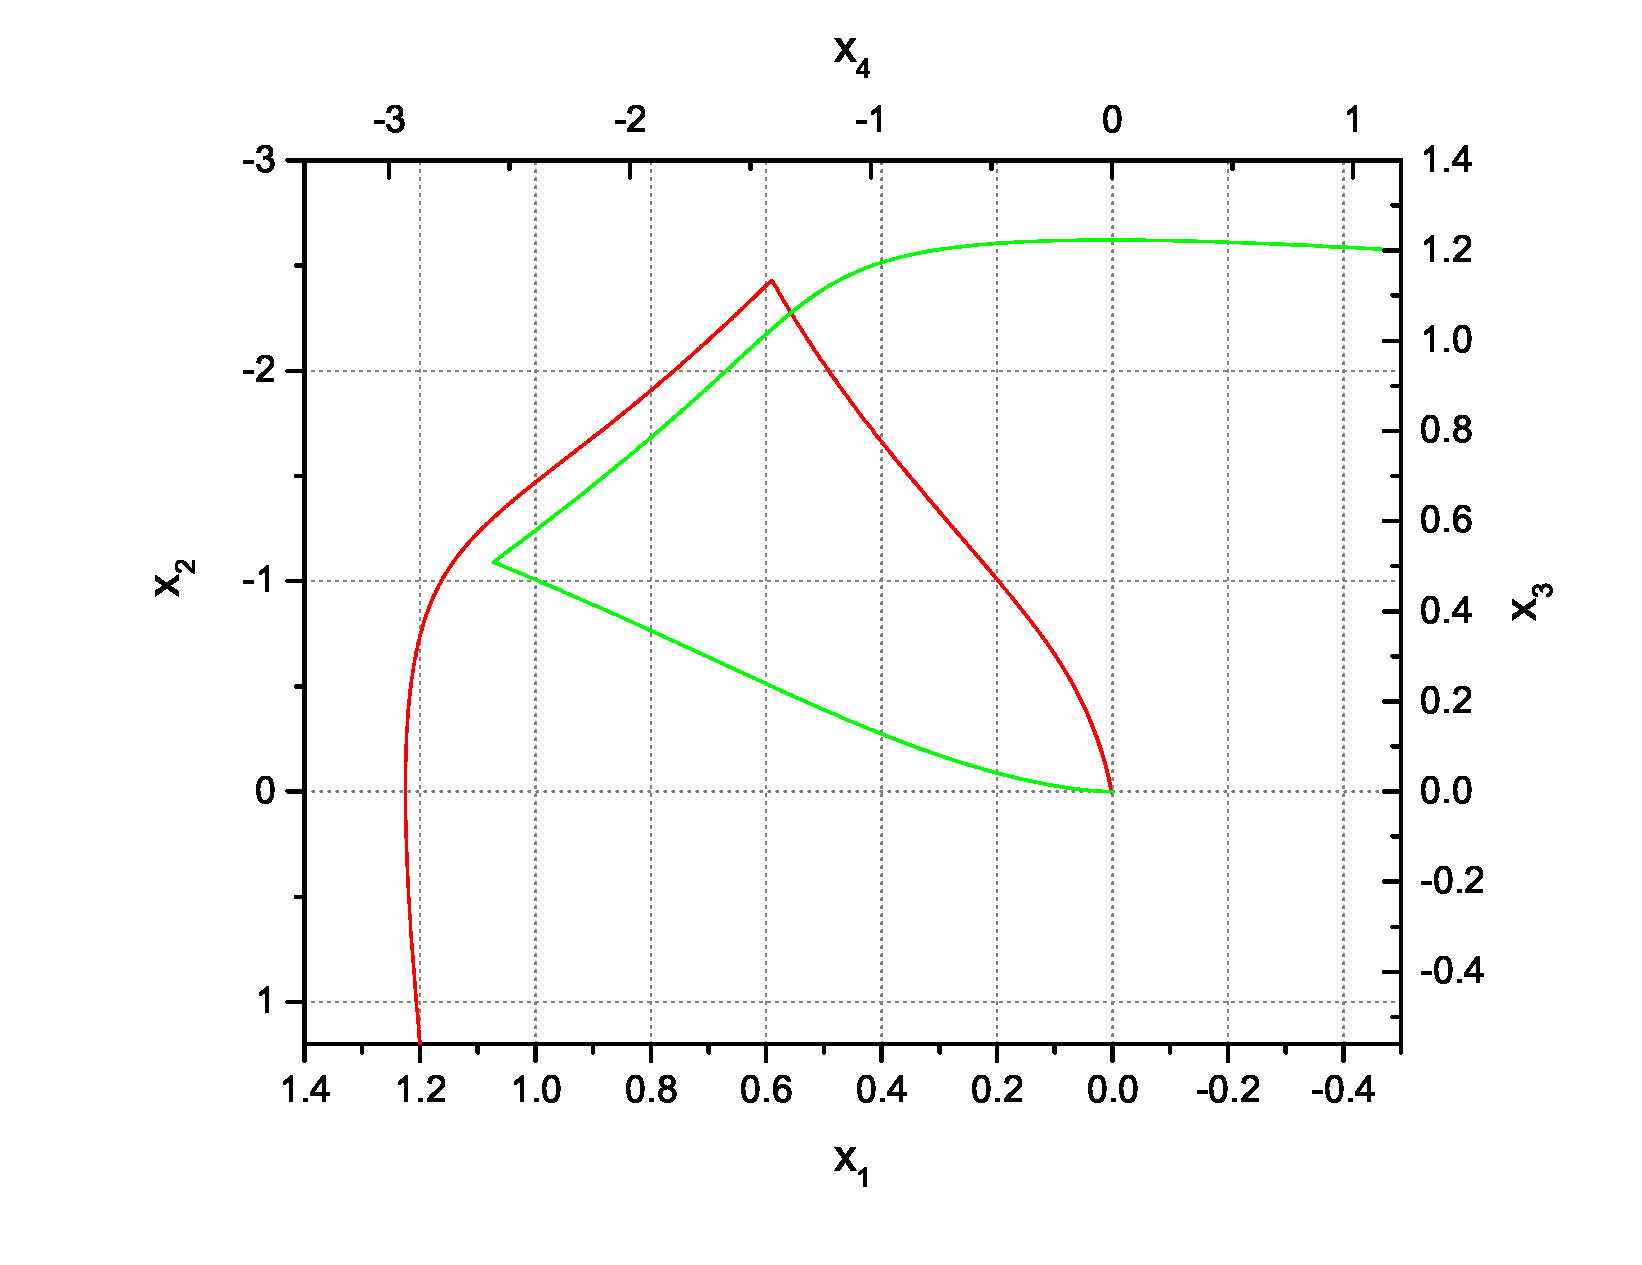
\includegraphics[width=0.7\textwidth]{paper3_fig2.eps}
\caption{Phase space trajectory}
\label{Figure:2}
\end{figure}

\begin{figure}
\centering
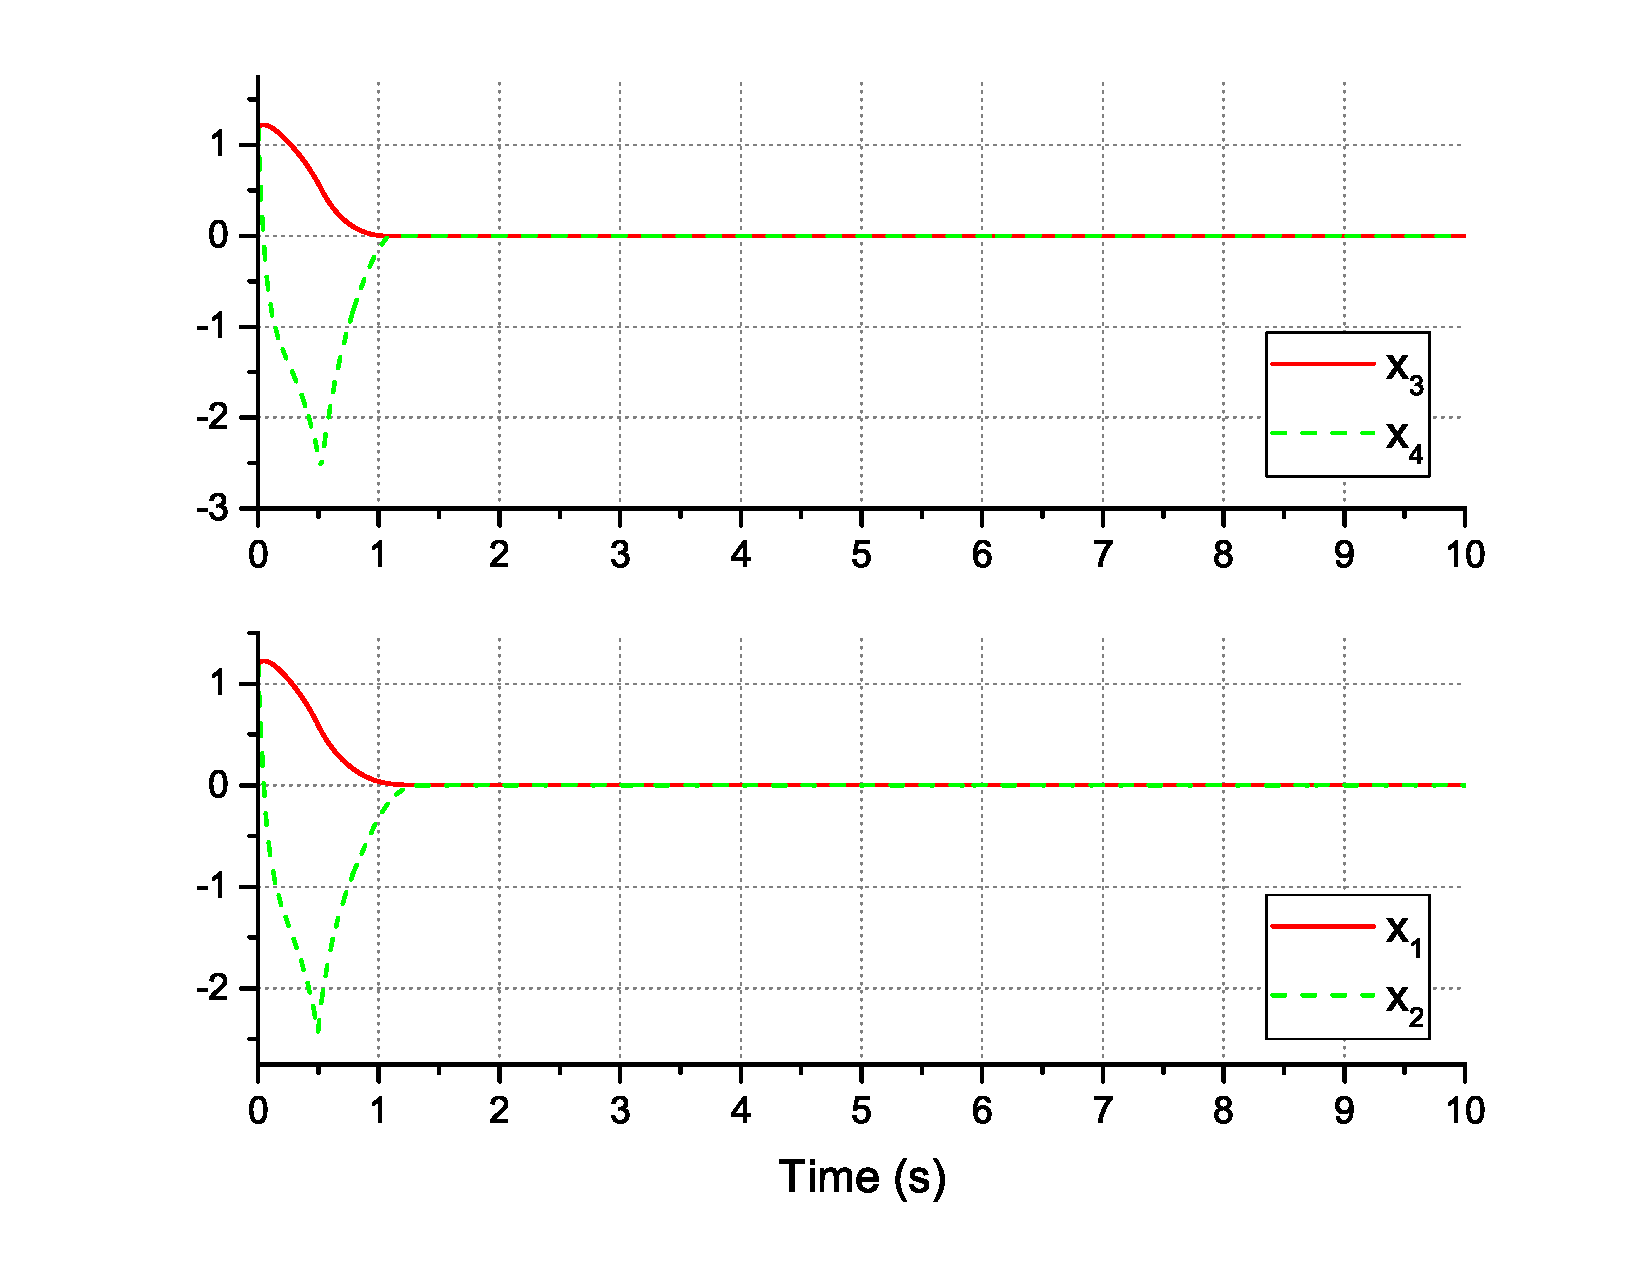
\includegraphics[width=0.7\textwidth]{paper3_fig2_20161108.eps}
\caption{system response}
\label{Figure:2_20161108}
\end{figure}

\begin{figure}
\centering
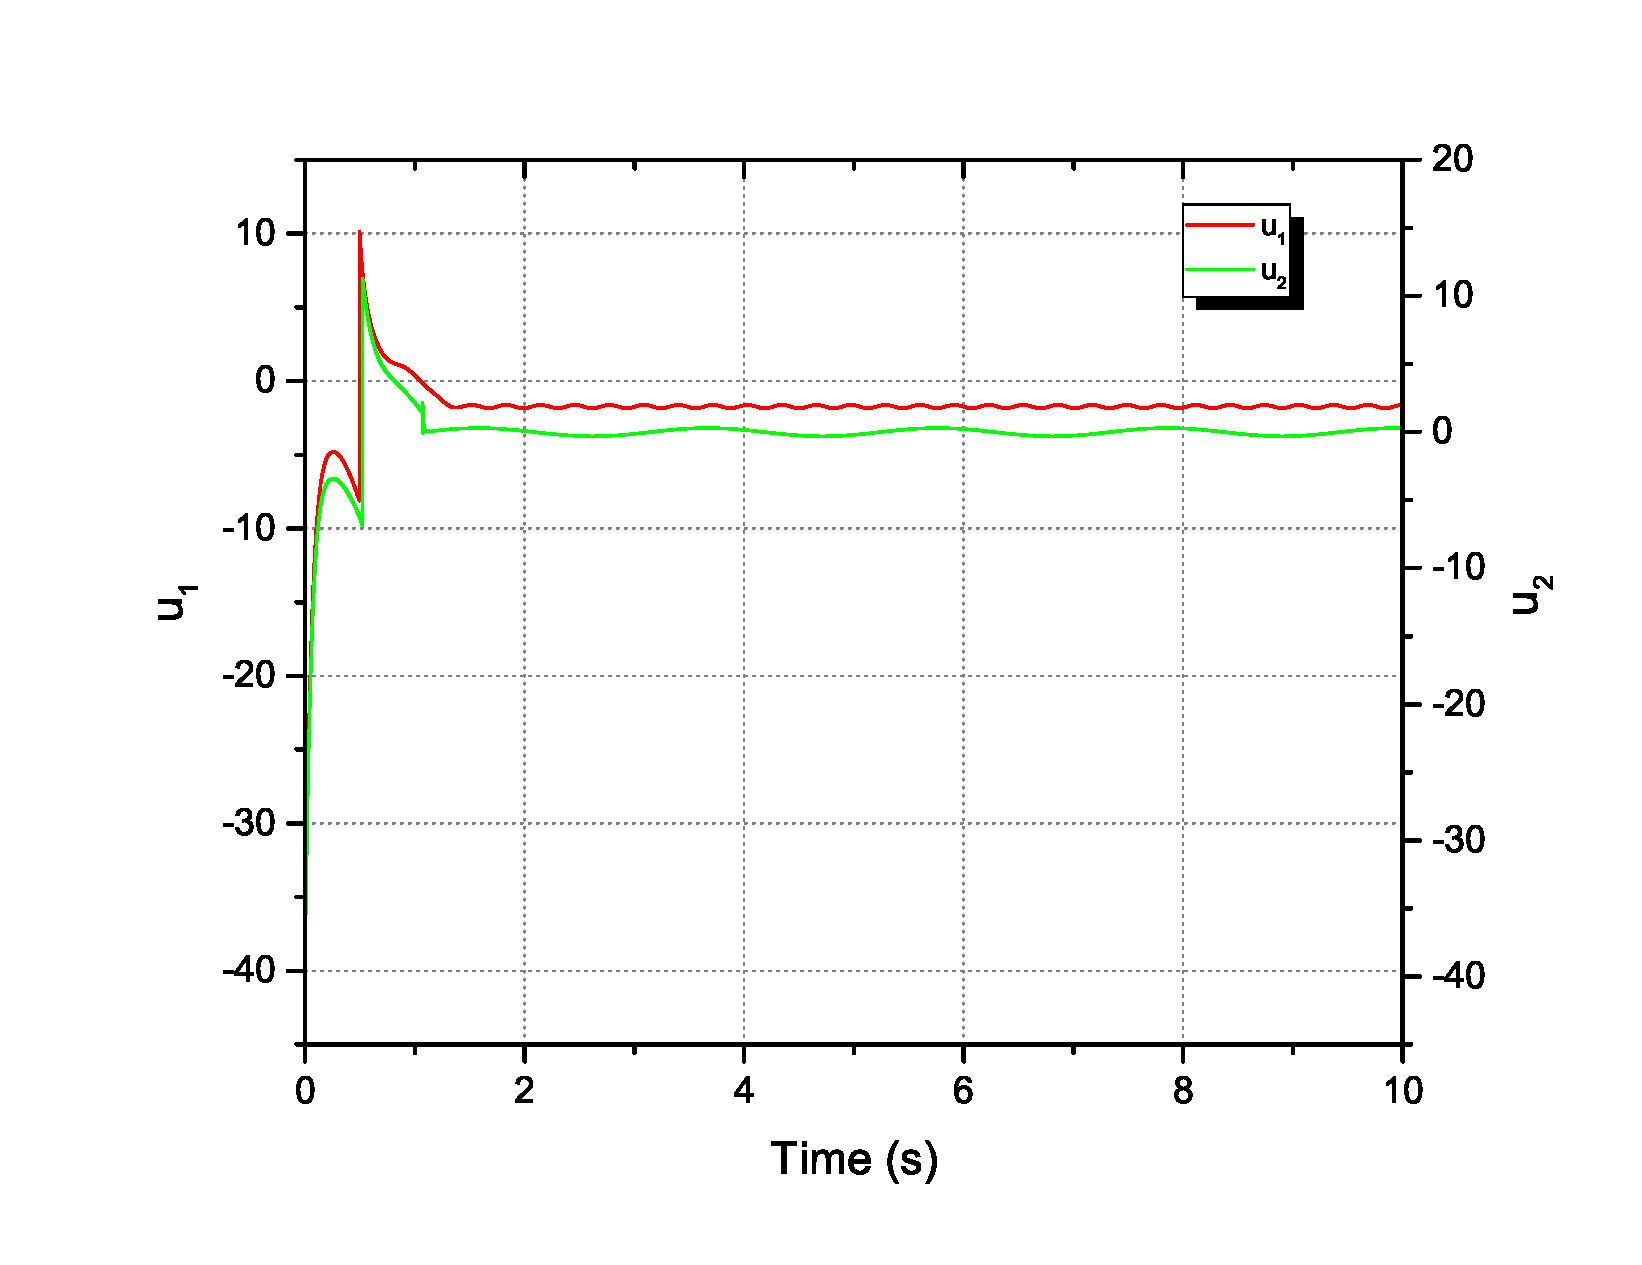
\includegraphics[width=0.7\textwidth]{paper3_fig3.eps}
\caption{System inputs}
\label{Figure:3}
\end{figure}
\subsection{Underactuated example}
Figure~\ref{Figure:8} shows an overhead crane system, the state space equations of which is same with the formula in Eq.~(\ref{eq:underactuated system}) with state variables selected as $\bm x=(x,\dot x,q,\dot q)$, and the details are listed:
\begin{align}
\begin{split}
f_1&=(M+m\sin^2q)^{-1}(mL\dot q^2\sin q+mg\sin q\cos q)\\
b_1&=(M+m\sin^2q)^{-1}\\
f_2&=-(ML+mL\sin^2q)^{-1}((M+m)g\sin q+mL\dot q^2\sin q\cos q)\\
b_2&=-(ML+mL\sin^2q)^{-1}\cos q,
\end{split}
\end{align}
where $x$ is defined as the displacement of the horizontal direction, and $q$ stands for the swing angle from the vertical line. $M=1kg$ and $m=0.8kg$ donate the masses of the trolley and the load in Figure~\ref{Figure:8}, respectively, and $g=9.8m/s^2$ refers to as the acceleration of gravity. $L=0.305m$ represents the length of the rope. In this simulation, the disturbances are also introduced:
\begin{align}
g_1(\bm x)&= 0.02\sin t\\
g_2(\bm x)&=0.07e^{-4t},
\end{align}
and those boundaries are easy to obtain. The initial condition of the overhead crane system is $\bm x_0 = (0.1,0,0.1,0)$, while the desired status is $\bm x_d = (2,0,0,0)$. The HDSM controller can be designed with the following set of parameters:
$c_1=1$, $c_2=4$, $\eta_u = 0.1$, $k_u=1$, $\gamma = 1$, $\lambda = 3$, $\alpha = 0.6$.\par
Figure~\ref{Figure:9} shows the state response curves of the overhead crane system controlled using the HDSM control scheme, and the results show that the controller stabilize the displacement at $6s$ approximately, though the disturbance exists in the system. One can find that the swing angle is fluctuating in a fairly small range, the boundary of which is not more than $1\times 10^-3rad$, hence this phenomena is reasonable and also occurs in the stable hierarchical sliding mode control \cite{wang2004design}.
\begin{figure}
\centering
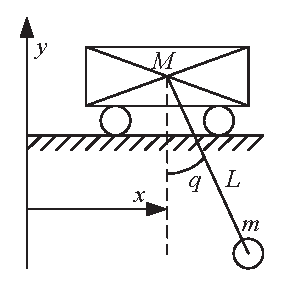
\includegraphics[width=0.3\textwidth]{paper3_fig8.eps}
\caption{Overhead crane schematic}
\label{Figure:8}
\end{figure}
\begin{figure}
\centering
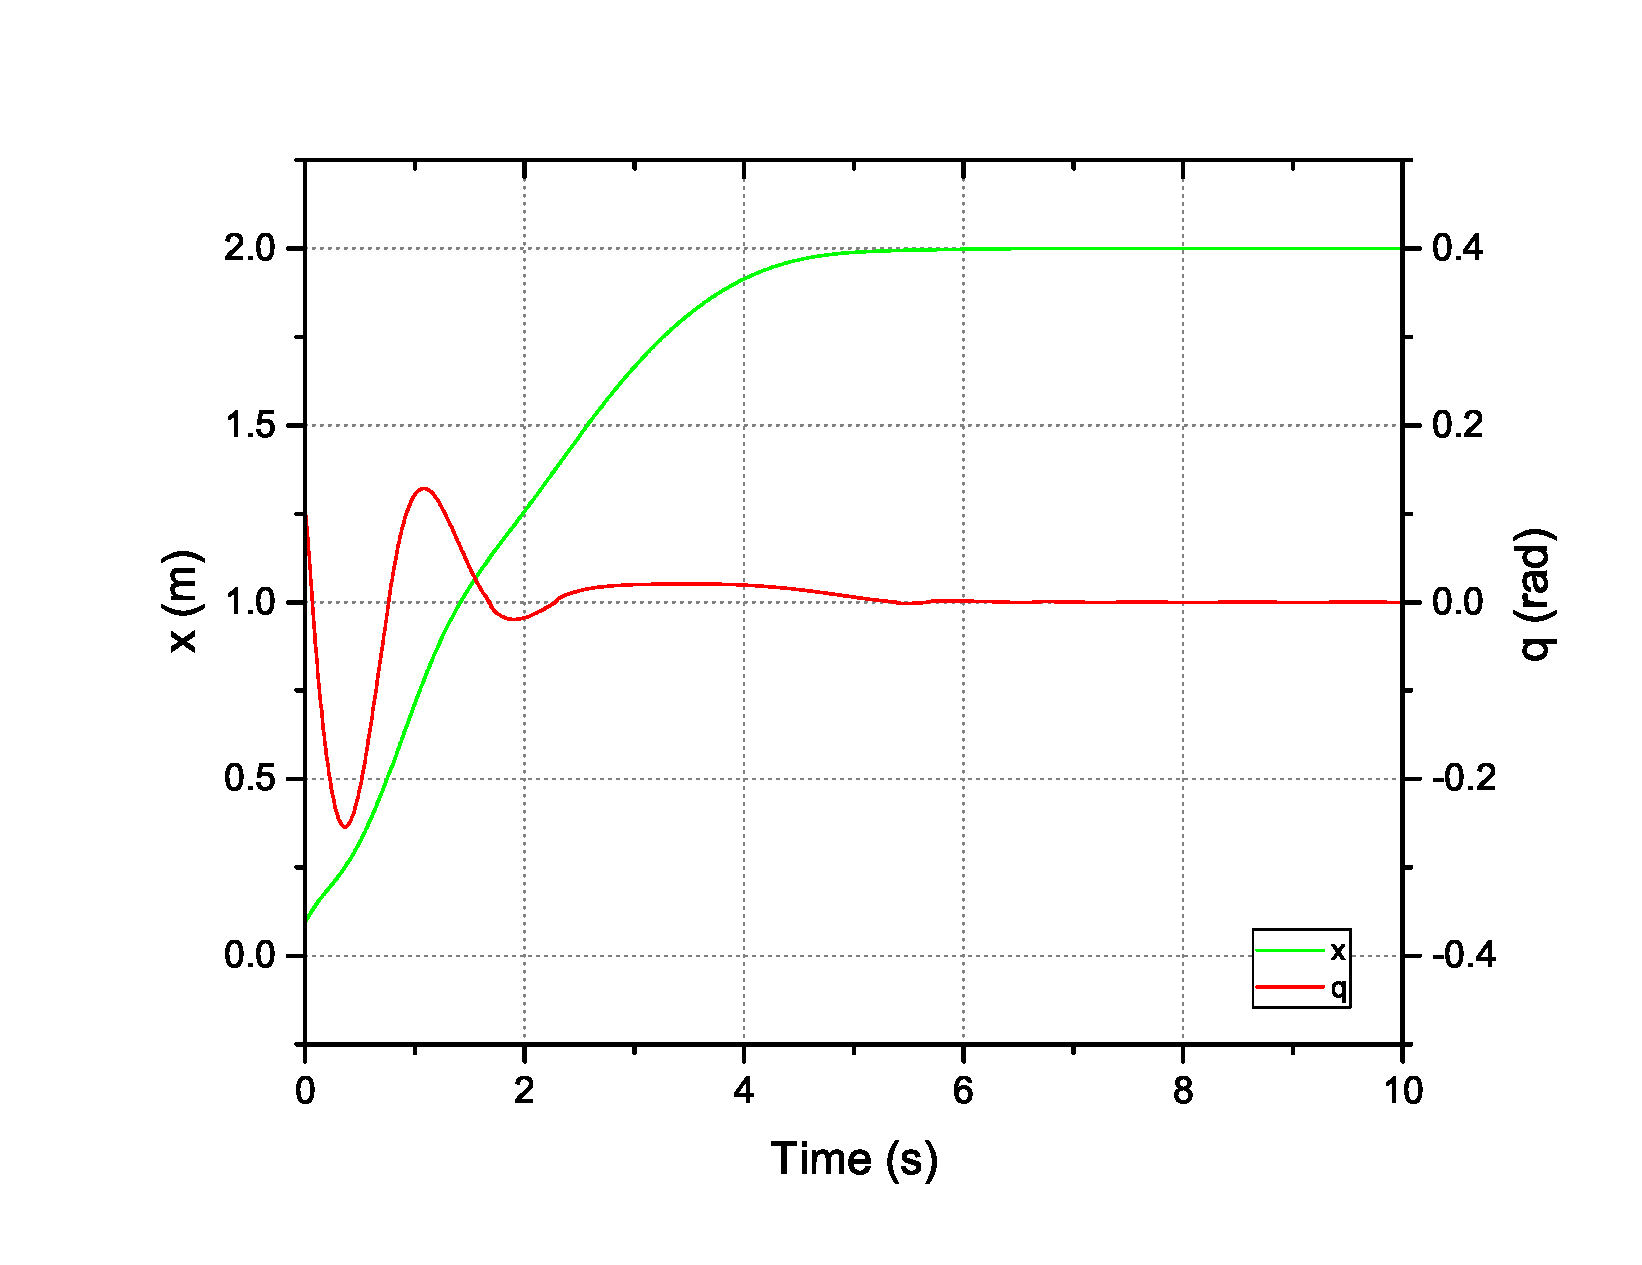
\includegraphics[width=0.7\textwidth]{paper3_fig9.eps}
\caption{Overhead crane dynamics}
\label{Figure:9}
\end{figure}
\subsection{Performance of the robotic manipulator}\label{sec:robotica manipulator}
In order to evaluate the performance of the proposed control scheme, a simulation about the $2$-link robotic manipulator is presented in the following context. Figure~\ref{Figure:1} is the $2$-link manipulator schematic, the dynamics of which can be explained by the dynamic equations in following forms:
\begin{figure}
\centering
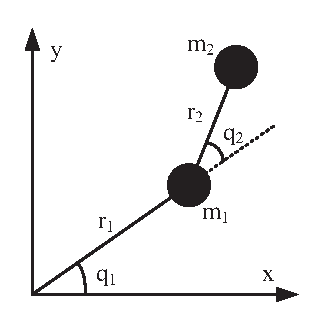
\includegraphics[width=0.3\textwidth]{paper3_fig1.eps}
\caption{$2$-link manipulator schematic}
\label{Figure:1}
\end{figure}

\begin{align}
\begin{bmatrix}
m_{12}(q_2) &m_{12}(q_2)\\
m_{21}(q_2) &m_{22}
\end{bmatrix}
\begin{pmatrix}
\ddot q_1\\
\ddot q_2
\end{pmatrix}
+
\begin{bmatrix}
-c(q_2)\dot q_1^2-2c(q_2)\dot q_1\dot q_2\\
c(q_2)\dot q_2^2
\end{bmatrix}+
\begin{bmatrix}
\xi_1(q_1,q_2) g\\
\xi_2(q_1,q_2) g
\end{bmatrix}=
\begin{pmatrix}
\tau_1\\
\tau_2
\end{pmatrix},
\end{align}
where
\begin{align*}
&m_{11}(q_2)=(m_1+m_2)r_1^2+m_2r_2^2+2m_2r_1r_2\cos(q_2)+J_1,\\
&m_{12}(q_2)=m_2r_2^2+m_2r_1r_2\cos(q_2),\\
&m_{21}(q_2)=m_{12}(q_2),\\
&m_{22}=m_2r_2^2+J_2,\\
&c(q_2)=m_2r_1r_2\sin(q_2),\\
&\xi_1(q_1,q_2) =(m_1+m_2)r_1\cos(q_2)+m_2r_2\cos(q_1+q_2),\\
&\xi_2(q_1,q_2) = m_2r_2\cos(q_1+q_2).
\end{align*}\par
The values of the parameters are listed here, $r_1=1m$, $r_2=0.8m$, $J_1=5 kgm$, $J_2=5kgm$, $m_1=0.5kg$, $m_2=1.5kg$. In this model, the uncertainty is brought in by estimated terms, namely, $\bar m_1=0.4$ and $\bar m_2=1.2$ which are all not the actual value obviously. In addition, owing to that it sits on many terms in the dynamic equations, it's a severe challenge to guarantee the performance. Accordingly, the uncertainty parameters in Eq.~(\ref{eq:manipulator uncertainty}) are assumed to be $\mu_0=10$, $\mu_1=3$, $\mu_2=3$.\par
This section will give a set of simulation to examine the performance of the MDTSM control in tracking the certain angle condition. The behavior of the manipulator should fulfill the initial and desired condition, namely, $(\bm q_0^T, \dot{\bm q}_0^T)= (0.3,0.2,0,0)$ and $({\bm q}_d^T,\dot{\bm q}_d^T)=(1,1,0,0)$. In order to ensure the stability and a fast convergence speed, the control parameters are chosen conservatively to make the manipulator track the desired attitude in finite time, and these parameters are $\alpha = 0.6$, $\gamma = 1$, $\lambda = 0.1$, $k = 150$. The terminal sliding mode control (TSM) scheme, as a comparison, is also implemented to regulate the behavior of the manipulator:
\begin{align}
\begin{split}
\bm s &= \dot{\bm \varepsilon}+C_\gamma\lceil\bm{sgn}^\alpha(\bm \varepsilon)\rfloor\\
\bm\tau &= \bm u_0+\bm u_1 +\bm u_2\\
\bm u_0 &= -M_0(\bm q)C_r\lceil\alpha\vert\bm\varepsilon\vert^{\alpha-1}\dot{\bm \varepsilon}\rfloor\\
\bm u_1 &= M_0(\bm q)\ddot {\bm q}_d+C_0(\bm q,\dot {\bm q})+g_0(\bm q)\\
\bm u_2 &= -k\frac{(\bm s^TM_0^{-1}(\bm q))^T}{\Vert\bm s^TM_0^{-1}(\bm q)\Vert}.
\end{split}
\end{align}
where the main control parameters of which are selected as $\alpha = 0.6$, $\gamma = 5$ and $k = 150$ to get a fairly good control performance.\par
The performance of the controllers mentioned above is illustrated in Figure~\ref{Figure:4} and Figure~\ref{Figure:5}. Comparatively speaking, $q_1$ reaches the desired state at about $3s$ with the MDTSM scheme, the reaching time of which is approximating $0.8s$ less than of the TSM scheme, and $q_2$ performs similar behaviors with a reasonable variable range of the angular rates. \textcolor{red}{From the results shown in Figure~\ref{Figure:4} and Figure~\ref{Figure:5}, we can find that the maximum theoretical finite convergence time $t_f=3.0843s$, which can be obtained directly accoring to Eq.~(\ref{eq:total convergence time}) and simulation datas, is more than $2.3s$, the convergence time of the simulation result. Hence, we can conclude that the results have verified the analyses about the convergence time in Section~\ref{sec:2}. For the MDTSM controller, the jiont~1 finishes its desired behaviour at about $2.3s$, and meanwhile the joint~2 spends about $1.6s$ completing the desired mission. Also, by observing the results, we can find that the stabilization time of the proposed method is less  than the TSM controller's, and the regulating process of the manipulators is steady and reasonable.} Therefore these results show that the MDTSM control scheme is able to achieve the regulation of the manipulator effectively.
\begin{figure}
\centering
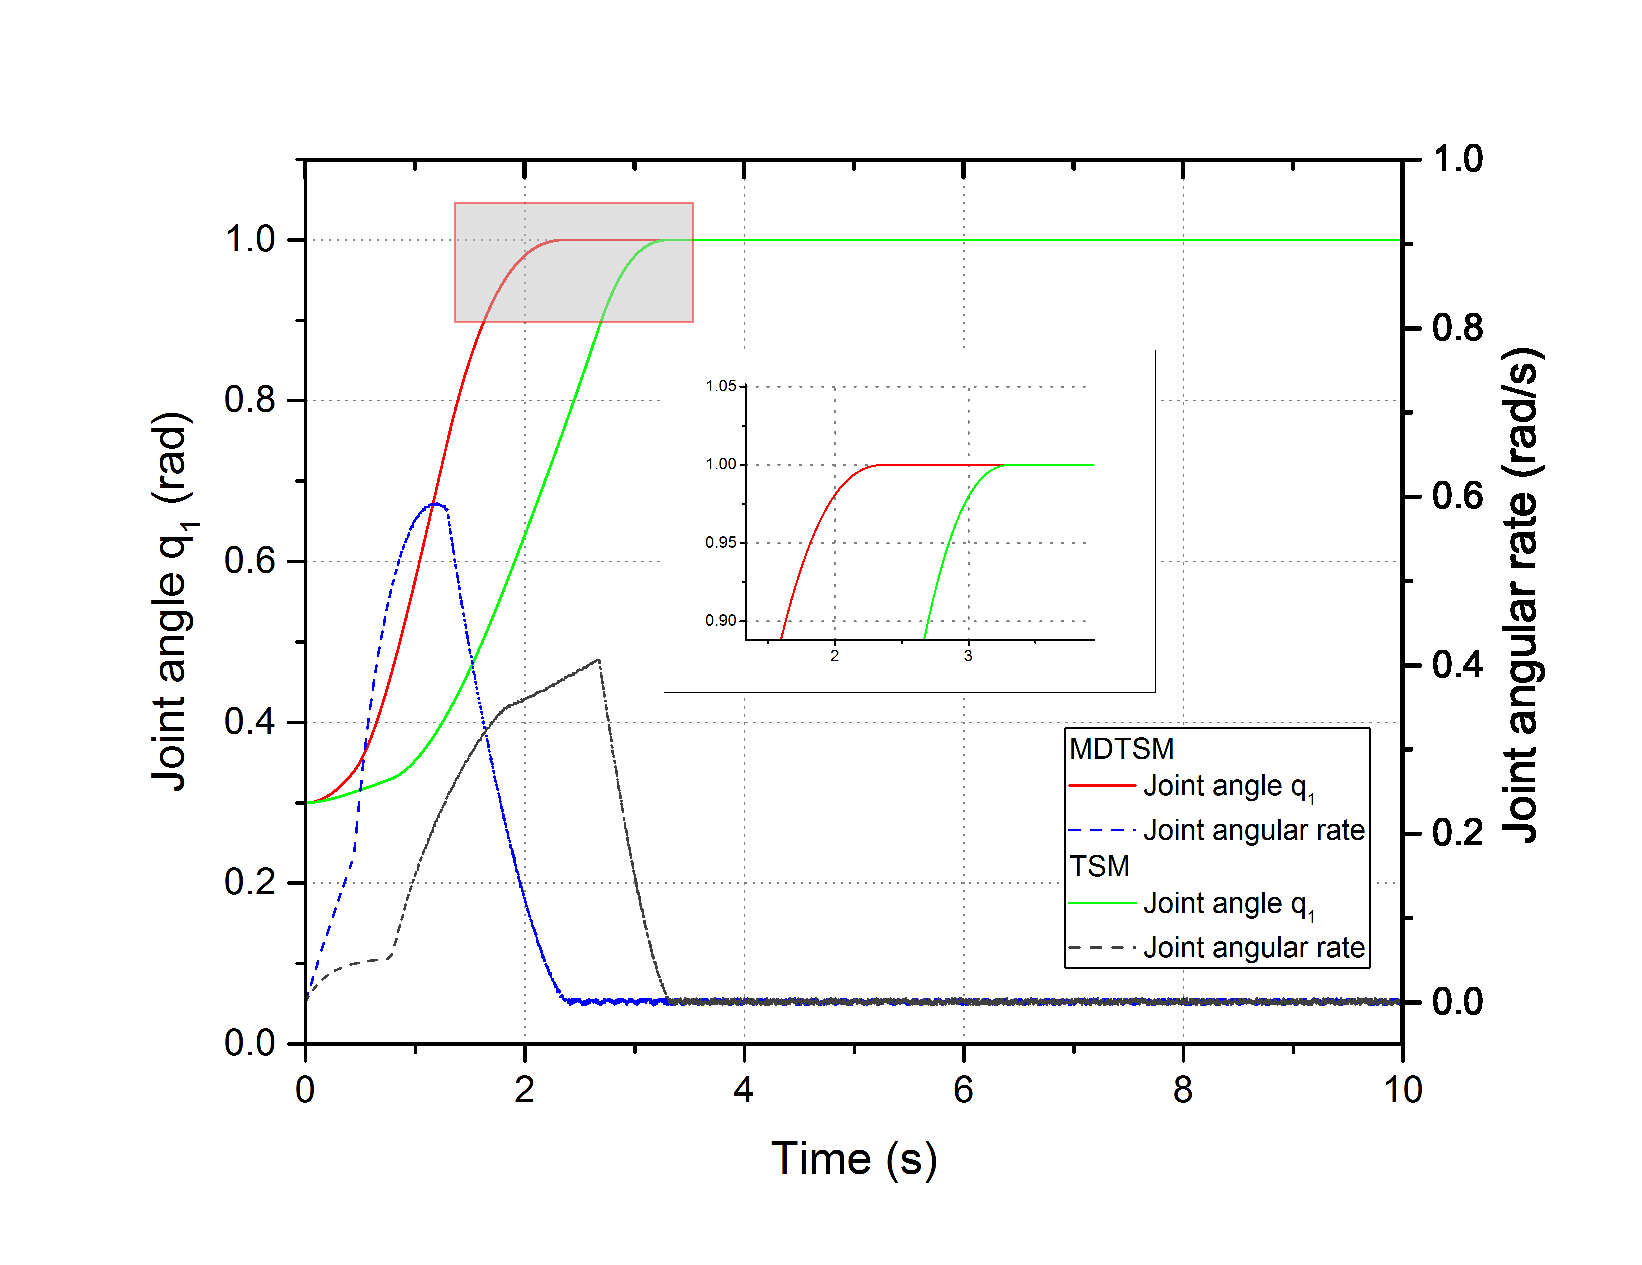
\includegraphics[width=0.7\textwidth]{paper3_fig4.eps}
\caption{Response of $q_1$ channel}
\label{Figure:4}
\end{figure}

\begin{figure}
\centering
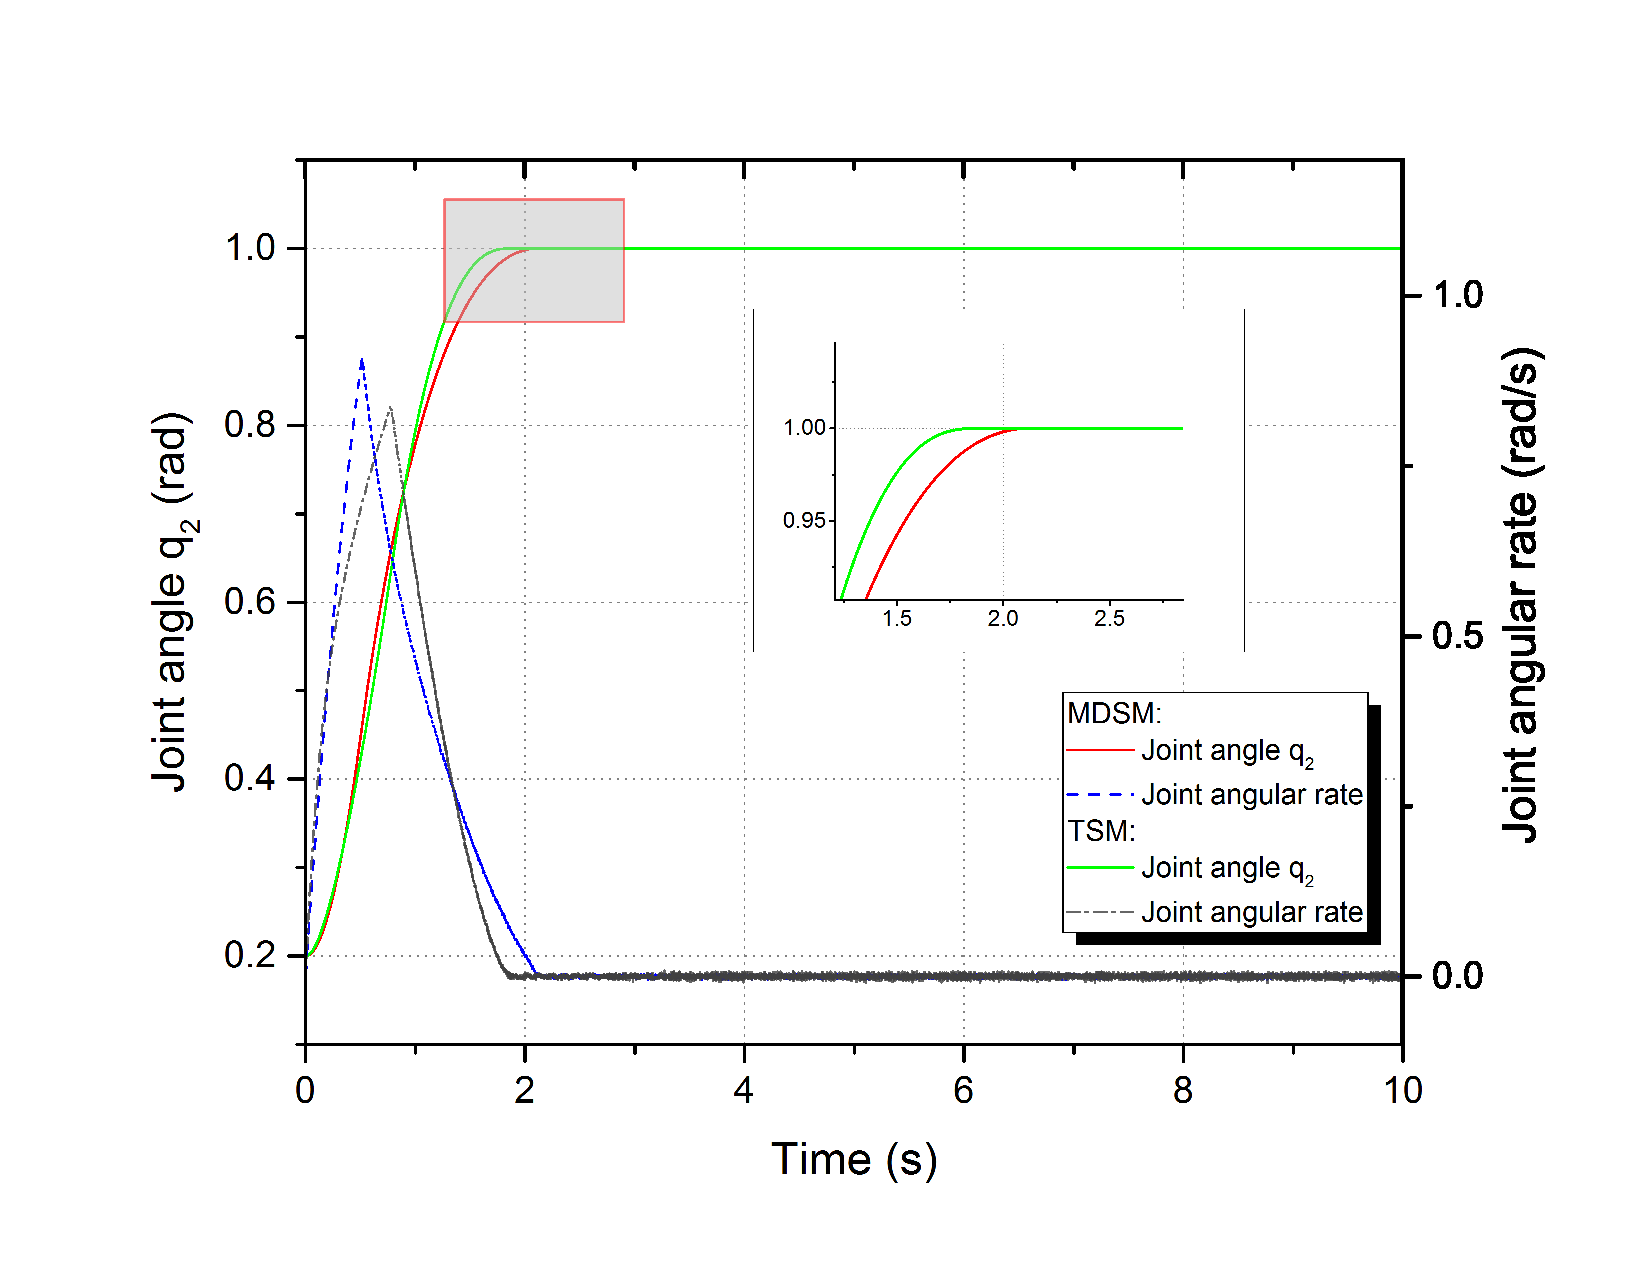
\includegraphics[width=0.7\textwidth]{paper3_fig5.eps}
\caption{Response of $q_2$ channel}
\label{Figure:5}
\end{figure}
The more general case, the robotic manipulator is usually required to track variable signal, is discussed in this section. Particularly, we continue to use the parameters of the controller mentioned above, and the mission condition is changed as follows:
\begin{align*}
&(\bm q_0^T, \dot{\bm q}_0^T)= (1.5,1.5,0,0)\\
&{\bm q}_d^T=(1.25-(1/5)e^{-t}+(1/20)e^{-4t},1.25+(9/40)e^{-t}-(1/4)e^{-2t})
\end{align*}\par
The simulation results are demonstrated in Figure~\ref{Figure:6} and Figure~\ref{Figure:7}, which plot the curves of states of the system~(\ref{eq:simulation second-order system}) regulated by adopting the MDTSM scheme. The control system completes the tracking mission at about $3.2s$ from a prescript initial condition, which performs a fairly small overshoot in the angle regulation.
\begin{figure}
\centering
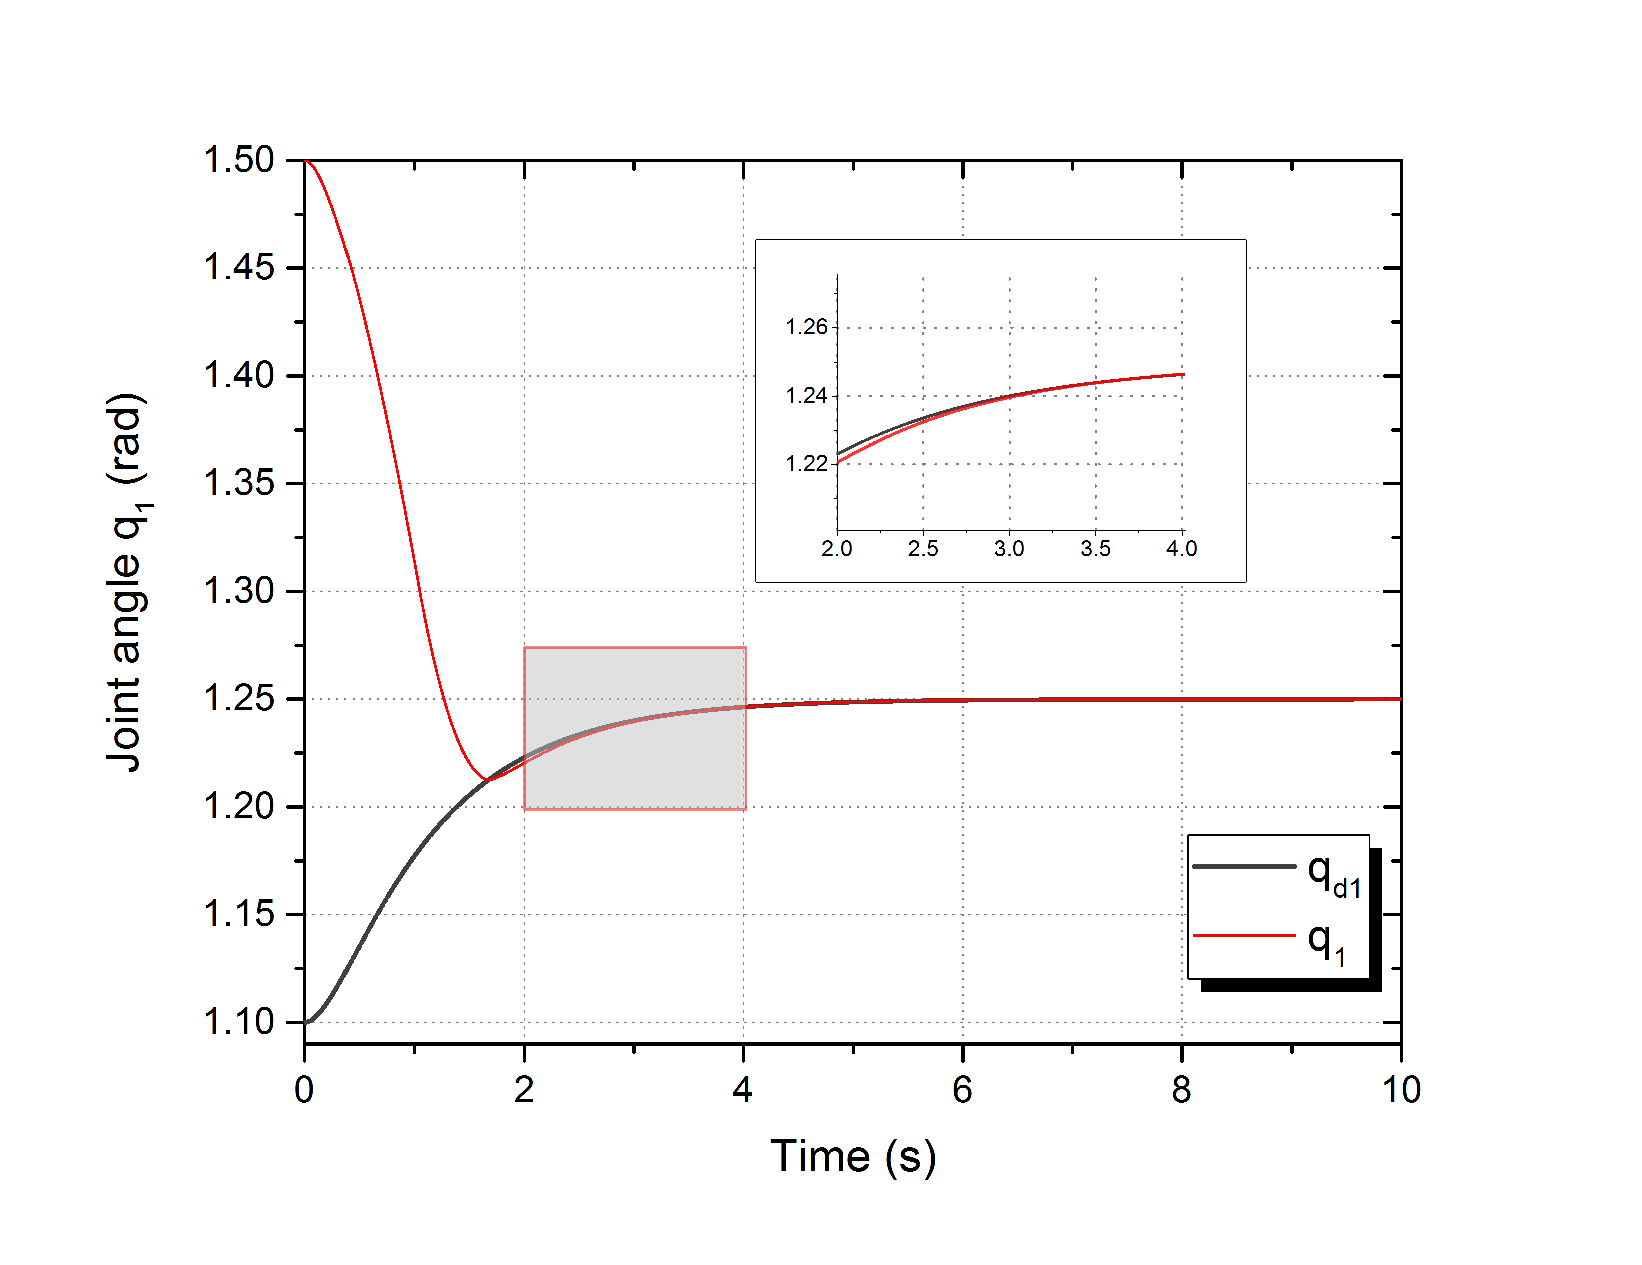
\includegraphics[width=0.7\textwidth]{paper3_fig6.eps}
\caption{Tracking performance of $q_1$ channel}
\label{Figure:6}
\end{figure}

\begin{figure}
\centering
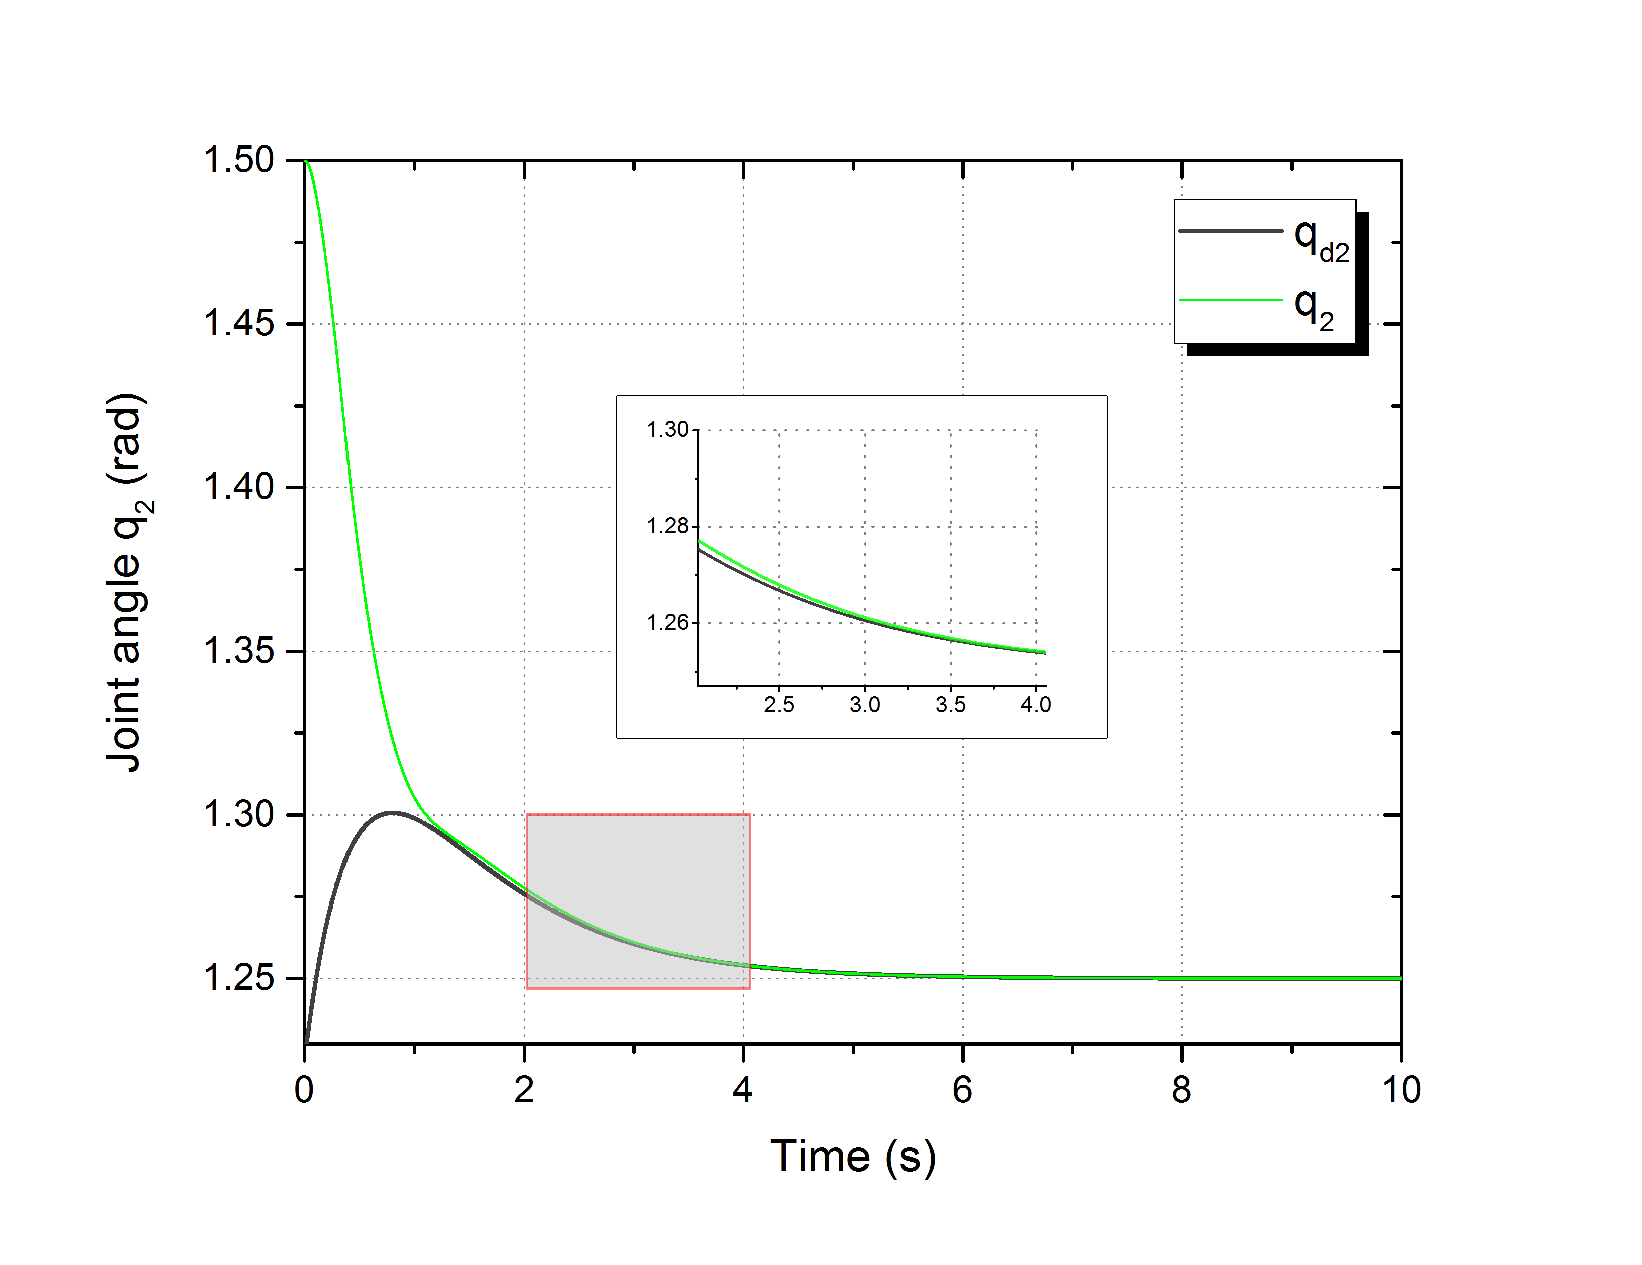
\includegraphics[width=0.7\textwidth]{paper3_fig7.eps}
\caption{Tracking performance of $q_2$ channel}
\label{Figure:7}
\end{figure}
\section{Conclusion}\label{sec:5}
A DTSM control for n-link robotic manipulator has been presented. The method integrates two individual subsystems as a unity, then builds the manifold and input for it to complete the controller design. The control scheme is able to guarantee the reaching condition of the desired sliding manifold, meanwhile the system states converge to the origin along the desired manifold. Also, the entire convergence time can be calculated accordingly. Developing the basic DTSM yields the MDTSM control, providing a solution to eliminating chattering, avoiding singularity and fast convergence. For dealing with the under actuated characteristics which may appear in the system, the HDTSM control is derived, and the overhead crane example verifies its effectiveness. However, the control parameters selection is still a challenge especially in the HDTSM scheme, and we will effort to excavate a full order dual terminal sliding mode methodology in the future for removing the obstacle caused by parameters essentially.
\section{Acknowledgment}
This work is partially supported by the National Natural Science Foundation of China (No. 61104112, 61503101).
\section{References}
\bibliography{paper3_ref}
\bibliographystyle{elsarticle-num}
\end{document}
